%!TEX TS-program = pdflatex
% paper.tex -- main diss file
%
% Wisconsin dissertation template
% Copyright (c) 2008-2009 William C. Benton.  All rights reserved.
%
% This program can redistributed and/or modified under the terms of the LaTeX
% Project Public License Distributed from CTAN archives in directory
% macros/latex/base/lppl.txt; either version 1 of the License, or (at your
% option) any later version.
%
% This program includes other software that is licensed under the terms of the
% LPPL and the Perl Artistic License; see README for details.
%
% You, the user, still hold the copyright to any document you produce with this
% software (like your dissertation).
%

%%% You'll want ``oneside'' for the deposit version, but probably not for any
%%% versions that don't need to meet the UW requirements
%%% MJG - note that the thesis dept updated the pt requirement from 12 to 10
%%% (2013)
\documentclass[10pt,oneside,letterpaper]{memoir}
\setlrmarginsandblock{1.1in}{*}{1}
\setulmarginsandblock{1.7in}{1in}{*}
\checkandfixthelayout

% preamble.tex -- packages to include
%
% Wisconsin dissertation template
% Copyright (c) 2008 William C. Benton.  All rights reserved.
%
% This program can redistributed and/or modified under the terms
% of the LaTeX Project Public License Distributed from CTAN
% archives in directory macros/latex/base/lppl.txt; either
% version 1 of the License, or (at your option) any later version.
%
% This program includes other software that is licensed under the
% terms of the LPPL and the Perl Artistic License; see README for details.
%
% You, the user, still hold the copyright to any document you produce
% with this software (like your dissertation).

%% Comment out any of these that you don't want
\usepackage{amssymb}
\usepackage{amsmath}
\usepackage{amsthm}
%\usepackage{theorem}
\usepackage{hyperref}

%%%%% LISTINGS package and setup
\IfFileExists{listings.sty}{%
\usepackage{listings}%
}{}

%% Packages added by Matt Gidden
%%
%% Note, order matters!
%%
\usepackage{cite} % right order for multiple entries in cite
\usepackage{moreverb} % for verbatim snippets of code
\usepackage{fancyvrb}
\usepackage{tabularx} % for tables with line breaks
\usepackage{threeparttable} % for tables with notes
\usepackage[capitalize, noabbrev]{cleveref} % for reference multiple figures
\usepackage{calc} % allows for arithmetic on latex variables
\usepackage{float} % allows for figures to be placed explicitly
\usepackage{algorithm2e} % for algorithms
\usepackage{subfig}
\usepackage{multirow} % combining rows in tables
\usepackage{footnote}
\usepackage{titlesec} % for using \titleformat
\usepackage{slashbox} % for tables with a divided cell, see http://tex.stackexchange.com/questions/7262/diagonally-divided-table-cell
\usepackage{bashful}
\usepackage{xspace}
\usepackage{color}
\definecolor{listinggray}{gray}{0.9}
\definecolor{lbcolor}{rgb}{0.9,0.9,0.9}
\lstset{
    %backgroundcolor=\color{lbcolor},
    language={C++},
    tabsize=4,
    rulecolor=\color{black},
    upquote=true,
    aboveskip={1.5\baselineskip},
    belowskip={1.5\baselineskip},
    columns=fixed,
    extendedchars=true,
    breaklines=true,
    prebreak=\raisebox{0ex}[0ex][0ex]{\ensuremath{\hookleftarrow}},
    frame=single,
    showtabs=false,
    showspaces=false,
    showstringspaces=false,
    basicstyle=\scriptsize\ttfamily\color{black},
    keywordstyle=\color[rgb]{0,0,1.0},
    commentstyle=\color[rgb]{0.133,0.545,0.133},
    stringstyle=\color[rgb]{0.627,0.126,0.941},
    numberstyle=\color[rgb]{0,1,0},
    identifierstyle=\color{black},
    captionpos=t,
}
\lstdefinestyle{BashOutputStyle}{
  basicstyle=\small\ttfamily,
  numbers=none,
  frame=tblr,
  columns=fullflexible,
  backgroundcolor=\color{blue!10},
  linewidth=0.9\linewidth,
  xleftmargin=0.1\linewidth
}
%
% Adding for some table features
\usepackage{array}
%
% Adding package for float barriers
\usepackage{placeins}

%% Custom commands added by Matt Gidden
\setcounter{tocdepth}{2}
\setcounter{secnumdepth}{3}
\theoremstyle{plain}
\newcommand{\Cyclopts}{\textsc{Cyclopts} }
\newcommand{\Cycamore}{\textsc{Cycamore} }
\newcommand{\cyclus}{\textsc{Cyclus}\xspace}
\newcommand{\Cyclus}{\textsc{Cyclus} }
\newcommand{\nucl}[2]{
\ensuremath{^{#1}}\mbox{#2}
}
\newcommand{\horizfig}[2][]{%
  \begin{minipage}{3in}\subfloat[#1]{#2}\end{minipage}}
%% \newcommand{\code}[1]{\lstinline[basicstyle=\ttfamily\color{green!40!black}]|#1|}
\newcommand{\code}[1]{\lstinline[basicstyle=\ttfamily\color{black}]|#1|}
\newcommand{\codeb}[1]{\texttt{#1}}
\newcommand{\units}[1] {\:\text{#1}}%
\newcommand{\citeme}{\textcolor{red}{CITE}\xspace}
\newcommand{\TODO}[1] {{\color{red}\textbf{TODO: #1}}}%
\newcommand{\Reactor}[1]{\texttt{Reactor{#1}}}
\newcommand{\UOXSource}{\texttt{UOX\_Source}}
\newcommand{\MOXSource}{\texttt{MOX\_Source}}
\newcommand{\Enrichment}{\texttt{Enrichment}}
\newcommand{\ffc}{$f_{\text{fc}}$\xspace}
\newcommand{\frx}{$f_{\text{rx}}$\xspace}
\newcommand{\floc}{$f_{\text{loc}}$\xspace}
\newcommand{\dloc}{$\delta_{\text{loc}}$\xspace}
\newcommand{\dreg}{$\delta_{\text{reg}}$\xspace}
\newcommand{\cbc}{Cbc\xspace}
\newcommand{\clp}{Clp\xspace}

%% You should use natbib
\IfFileExists{natbib.sty}{%
  \usepackage[numbers]{natbib}% added the numbers option from the original WI
                              % thesis template
}{}

%% You probably need appendix, if you want appendices
\IfFileExists{appendix.sty}{%
\usepackage{appendix}%
}{}

%% the spacing in memoir is weird, you'll need to use this
\DisemulatePackage{setspace}
\usepackage[onehalfspacing]{setspace}

%% List setup; the ``hanglist`` environment will allow you to have
%% nicely-typeset enumerated lists (i.e., with the numbers hanging in
%% the margins).  You need at least version 2.1 of enumitem.sty.  If
%% you don't have enumitem installed at all, hanglist will just be an
%% alias for enumerate.
\IfFileExists{enumitem.sty}{%
\usepackage[loadonly]{enumitem}[2007/06/30]%
\newlist{hanglist}{enumerate}{1}% 
\setlist[hanglist]{label=\arabic*.}%
\setlist[hanglist,1]{leftmargin=0pt}%
}{%
\newenvironment{hanglist}{\begin{enumerate}}{\end{enumerate}}%
}

\IfFileExists{mathpartir.sty}{%
\usepackage{mathpartir}%
}{}

%% \newtheorem{thm}{Theorem}[chapter] % reset theorem numbering for each chapter
%% \theoremstyle{definition}
%% \newtheorem{defn}[thm]{Definition} % definition numbers are dependent on theorem numbers
%% \newtheorem{exmp}[thm]{Example} % same for example numbers


%% Get rid of ugly borders around PDF hyperlinks (e.g., for cross-references, bib entries, or URLs)
\hypersetup{pdfborder = 0 0 0}

%% You want microtype.
\IfFileExists{microtype.sty}{%
\usepackage[protrusion=true,expansion=true]{microtype}%
}{}

%\pagestyle{thesisdraft}

% Surround parts of graphics with box
\usepackage{boxedminipage}

%% booktabs (thx to Nate Rosenblum for bringing this beautiful package
%% to my attention)
\IfFileExists{booktabs.sty}{%
\usepackage{booktabs}%
}{}

% This is now the recommended way for checking for PDFLaTeX:
\usepackage{ifpdf}

%% Avoid ugly "Type 3" fonts
\usepackage{lmodern}
\usepackage[LY1]{fontenc}

%% Substitute your favorite serif and sans fonts here....
\IfFileExists{tgpagella.sty}{%
% TeX Gyre pagella, like Palatino
\usepackage{tgpagella}%
}{}

%% overrides the default Latex math font with AMS Euler
%\usepackage[LY1]{eulervm} 

\ifpdf
\usepackage[pdftex]{graphicx}
\else
\usepackage{graphicx}
\fi

\usepackage{makeidx}
\makeindex

{\theoremstyle{plain}
\newtheorem{thm}{Theorem}[chapter]
\newtheorem{cor}[thm]{Corollary}
\newtheorem{define}[thm]{Definition}
\newtheorem{exmpl}[thm]{Example}
}
{\theoremstyle{remark}
\newtheorem{rmk}[thm]{Remark}
}

\newtheoremstyle{customsty1}
{3pt}%
{3pt}%
{}% --- body font
{}% --- indent amount
{\bfseries}% --- Theorem head font
{:}% --- Punctuation after head
{.5em}% --- space after head
{}% --- theorem head spec (can be left empty, meaning 'normal')

% Define 'newtheorems' that use ``customsty1''
{\theoremstyle{customsty1} 
}


%%% NB: the ``deposit'' chapter- and page- styles should conform to UW
%%% requirements.  If you are producing a pretty version of your
%%% dissertation for web use later, you will certainly want to make
%%% your own chapter and page styles.

\makechapterstyle{deposit}{%
  \renewcommand{\chapterheadstart}{}
  \renewcommand{\printchaptername}{}
  \renewcommand{\chapternamenum}{}
  \renewcommand{\printchapternum}{\parbox{2em}{\MakeLowercase{\Large\scshape\thechapter{}}} }
  \renewcommand{\afterchapternum}{}
  \renewcommand{\printchaptertitle}[1]{%
  \raggedright\Large\scshape\MakeLowercase{##1}}
  \renewcommand{\afterchaptertitle}{%
  \vskip\onelineskip \hrule\vskip\onelineskip}
}

\makepagestyle{deposit}
 
\makeatletter
 
\renewcommand{\chaptermark}[1]{\markboth{#1}{}}
\renewcommand{\sectionmark}[1]{\markboth{#1}{}}
 
\makeevenfoot{deposit}{}{}{}
\makeoddfoot{deposit}{}{}{}
\makeevenhead{deposit}{\thepage}{}{}
\makeoddhead{deposit}{}{}{\thepage}
\makeatother

%%% set up page numbering for chapter pages to satisfy UW requirements
%%% NB: You will want to delete until the ``SNIP'' mark if you are
%%% making a ``nice'' copy
\copypagestyle{chapter}{plain}
\makeoddfoot{chapter}{}{}{}
\makeevenhead{chapter}{\thepage}{}{}
\makeoddhead{chapter}{}{}{\thepage}
%%% SNIP

%%% bib nonsense
\makeatletter
\newenvironment{wb-bib}[1]{%
  \chapter*{references}
\ifnobibintoc\else 
\phantomsection 

\addcontentsline{toc}{chapter}{References } 
\fi 
\prebibhook
  \begin{bibitemlist}{#1}}{\end{bibitemlist}\postbibhook}

\AtBeginDocument{%
  \@ifpackageloaded{natbib}{% natbib is loaded
    \addtodef{\endthebibliography}{}{\vskip-\lastskip\postbibhook}
    \@ifpackagewith{natbib}{sectionbib}{% with sectionbib option
      \renewcommand{\bibsection}{\@memb@bsec}}%
      {\renewcommand{\bibsection}{\@memb@bchap}}}%
  {}
  \@ifpackagewith{chapterbib}{sectionbib}{%
    \renewcommand{\sectionbib}[2]{}
    \renewcommand{\bibsection}{\@memb@bsec}}{}
}
\makeatother

% defs.tex -- wbepi environment for chapter epigraphs and other useful defs.
%
% Wisconsin dissertation template
% Copyright (c) 2008 William C. Benton.  All rights reserved.
%
% This program can redistributed and/or modified under the terms
% of the LaTeX Project Public License Distributed from CTAN
% archives in directory macros/latex/base/lppl.txt; either
% version 1 of the License, or (at your option) any later version.
%
% This program includes other software that is licensed under the
% terms of the LPPL and the Perl Artistic License; see README for details.
%
% You, the user, still hold the copyright to any document you produce
% with this software (like your dissertation).


%% put lstnewenvironment declarations here, if you're using listings

%% end lstnewenvironment declarations

%% I put convenience definitions that will go in several chapters here

%%%%% begin convenience definitions

\makeatletter
\newcommand{\wb@episource}{}
\newenvironment{wbepi}[1]{\begin{quote}\renewcommand{\wb@episource}{#1}\itshape}{\par\upshape \raggedleft --- \textsc{\wb@episource}\\ \end{quote}}
\makeatother

%%%%% SVN
\IfFileExists{svn-multi.sty}{%
\usepackage{svn-multi}%
%%% Uncomment the second one and comment out the first one if you want
%%% to include subversion revision information in each file.
\newcommand{\vcinfo}{}%
%\newcommand{\vcinfo}{\begin{centering}\fbox{\fbox{\parbox{5in}{Author: \svnauthor\\Revision: \svnfilerev\\Last changed on: \svnfiledate\\URL: \svnkw{HeadURL}}}}\\[1em]\end{centering}}%
}{%
\newcommand{\svnidlong}[4]{}%
\newcommand{\svnfilerev}{}%
\newcommand{\svnauthor}{}%
\newcommand{\svnfiledate}{}%
\newcommand{\svnkw}{}%
\newcommand{\vcinfo}{}%
}

%%%%% end convenience definitions

% thesisdefs.tex

% This is mostly adapted from withesis.cls.  The original copyright
% notice for withesis.cls follows, preceded by two percent signs (%%):

%% withesis.cls
%% LaTeX Style file for the University of Wisconsin-Madison Thesis Format
%% Adapted from the Purdue University Thesis Format
%% Originally by Dave Kraynie
%% Edits by Darrell McCauley
%% Adapted to UW-Madison format by Eric Benedict  (Noted with <EB>)
%% Updated to LaTeX2e by Eric Benedict 24 July 00
%% 
%%=============================================================================
%% Licensed under the Perl Artistic License.
%% see: http://www.ctan.org/tex-archive/help/Catalogue/licenses.artistic.html
%% for more info...
%%=============================================================================

% withesis.cls is available from CTAN.  The modifications to this file
% are also licensed under the Perl Artistic License.

% --wb, 2008

\makeatletter

\newcounter {tocpage}
\newcounter {lofpage}
\newcounter {lotpage}
\newcounter {listofheading}

\newcommand\@thesistitlemedskip{0.2in}
\newcommand\@thesistitlebigskip{0.6in}
\newcommand{\degree}[1]{\gdef\@degree{#1}}
\newcommand{\project}{\gdef\@doctype{A masters project report}}
\newcommand{\prelim}{\gdef\@doctype{A preliminary report}}
\newcommand{\thesis}{\gdef\@doctype{A thesis}}
\newcommand{\dissertation}{\gdef\@doctype{A dissertation}}
\newcommand{\department}[1]{\gdef\@department{(#1)}}

\newenvironment{titlepage}
 {\@restonecolfalse\if@twocolumn\@restonecoltrue\onecolumn
  \else \newpage \fi \thispagestyle{empty}
% \c@page\z@ -- deleted: count title page in thesis
}{\if@restonecol\twocolumn \else \newpage \fi}

\gdef\@degree{Doctor of Philosophy}    %Default is PhD
\gdef\@doctype{A dissertation}         %Default is dissertation

\gdef\@department{(Nuclear Engineering and Engineering Physics)}
\gdef\@defensedate{03/26/2015}
\gdef\@committee{
  \hspace*{1cm}Michael L. Corradini, Professor, Nuclear Engineering and Engineering Physics\\
  \hspace*{1cm}James R. Luedtke, Professor, Industrial and Systems Engineering\\
  \hspace*{1cm}Laura A. McLay, Professor, Industrial and Systems Engineering\\
  \hspace*{1cm}Erich A. Schneider, Professor, Nuclear Engineering, University of Texas at Austin\\
  \hspace*{1cm}Paul P.H. Wilson, Professor, Nuclear Engineering and Engineering Physics
  %<+Name+>, <+Title+>, <+Department+>\\
  } 

\renewcommand{\maketitle}{%
  \begin{titlepage}
%-----------------------------------------------------------------------------
% -- The thesis office doesn't like thanks on title page.  Put it in
% -- the acknowledgments.  This is here so you don't have to change
% -- your titlepage when converting from report style. -> from Purdue, but I
%        left it here since it seems compatible with UW-Madison, Eric
%-----------------------------------------------------------------------------
    \def\thanks##1{\typeout{Warning: `thanks' deleted from thesis titlepage.}}
    \let\footnotesize\small \let\footnoterule\relax \setcounter{page}{1}
    \begin{center}
      {\textbf{\expandafter\expandafter{\@title}}} \\[\@thesistitlebigskip]
       by \\[\@thesistitlemedskip]
      \@author \\[\@thesistitlebigskip]
      \@doctype\ submitted in partial fulfillment of \\
      the requirements for the degree of\\[\@thesistitlebigskip]
      \@degree \\[\@thesistitlemedskip]
      \@department \\[\@thesistitlebigskip]
      at the \\[\@thesistitlemedskip]
      UNIVERSITY OF WISCONSIN--MADISON\\[\@thesistitlemedskip]
      \@date
      \\[\@thesistitlemedskip]
    \end{center}
  %% for final thesis
  %% with large margins
  Date of final oral examination: \@defensedate \\[\@thesistitlemedskip]
  The dissertation is approved by the following members of the Final Oral Committee:\\
  %%
  \@committee
  \end{titlepage}
  \setcounter{footnote}{0}
  \setcounter{page}{1} %title page is NOT counted
  \let\thanks\relax
  \let\maketitle\relax \let\degree\relax \let\project\relax \let\dissertation\relax
  \let\department\relax
  \gdef\@thanks{}\gdef\@degree{}\gdef\@doctype{}
  \gdef\@department{}
  %\gdef\@author{}\gdef\@title{}
}


%=============================================================================
% ABSTRACT
%=============================================================================
% The abstract should begin with two single-spaced lines describing
% the author and title in a standard format.  After these lines comes
% the standard abstract.
%=============================================================================
\def\abstract{
  \chapter*{Abstract}
  \addcontentsline{toc}{chapter}{Abstract}
  \relax\markboth{Abstract}{Abstract}}
\def\endabstract{\par\newpage}


%=============================================================================
% UMI ABSTRACT
%=============================================================================
% The UMI abstract should begin with the author and title in a standard format.
% After the author comes the advisor and university. After these lines comes
% a bunch of double spaced text to make up the standard abstract.
% After the abstract, the advisor's approval signature follows.
% This page is not numbered and is delivered seperately to the thesis office.
%=============================================================================

\def\advisortitle#1{\gdef\@advisortitle{#1}}
\def\advisorname#1{\gdef\@advisorname{#1}}
\gdef\@advisortitle{Professor}
\gdef\@advisorname{Cheer E.\ Place}

\def\umiabstract{
             \thispagestyle{empty}
                  \addtocounter{page}{-1}
                \begin{center}
                  {\textbf{\expandafter\uppercase\expandafter{\@title}}}\\
                  \vspace{12pt}
                  \@author \\
                  \vspace{12pt}
                  Under the supervision of \@advisortitle\ \@advisorname\\
                  At the University of Wisconsin-Madison
                \end{center}
}

\def\endumiabstract{\vfill \hfill\@advisorname\par\newpage}


%============================================================================
% VERBATIMFILE
%============================================================================
% \verbatimfile{<filename>}    for verbatim inclusion of a file
% - Note that the precise layout of line breaks in this file is important!
% - added the \singlespace - EB
%============================================================================
\def\verbatimfile#1{\begingroup \singlespace
                    \@verbatim \frenchspacing \@vobeyspaces
                    \input#1 \endgroup
}


%=============================================================================
% SEPARATOR Pages
%   Creates a blank page with a text centered horizontally and vertically.
%   The page is neither counted nor numbered.
%   These pages are required in the thesis format before sections such
%   as appendices, vita, bibliography, etc.
%=============================================================================
\def\separatorpage#1{
  \newpage
  \thispagestyle{empty}
  \addtocounter{page}{-1}
  \null
  \vfil\vfil
  \begin{center}
    {\textbf{#1}}
  \end{center}
  \vfil\vfil
  \newpage}


%=============================================================================
% COPYRIGHTPAGE
%=============================================================================
% The copyright must do the following:
% - start a new page with no number
% - place the copyright text centered at the bottom.
%=============================================================================
\def\copyrightpage{
  \newpage
  \thispagestyle{empty}    % No page number
  \addtocounter{page}{-1}
  \chapter*{}            % Required for \vfill to work
  \begin{center}
   \vfill
   \copyright\ Copyright by \@author\ \@date\\
   All Rights Reserved
  \end{center}}


%=============================================================================
% GLOSSARY
%=============================================================================
% The glossary environment must do the following:
% - produce the table of contents entry for the glossary
% - start a new page with GLOSSARY centered two inches from the top
%=============================================================================
\def\glossary{
  \chapter*{GLOSSARY}
  \addcontentsline{toc}{chapter}{Glossary}}
\def\endglossary{\par\newpage}

%=============================================================================
% NOMENCLATURE
%=============================================================================
% The nomenclature environment must do the following:
% - produce the table of contents entry for the nomenclature section
% - start a new page with NOMENCLATURE centered two inches from the top
%=============================================================================
\def\nomenclature{\separatorpage{DISCARD THIS PAGE}
  \chapter*{Nomenclature}
  \addcontentsline{toc}{chapter}{NOMENCLATURE}}
\def\endnomenclature{\par\newpage}

%=============================================================================
% CONVENTIONS
%=============================================================================
% The conventions environment must do the following:
% - produce the table of contents entry for the nomenclature section
% - start a new page with CONVENTIONS centered two inches from the top
%=============================================================================
\def\conventions{\separatorpage{DISCARD THIS PAGE}
  \chapter*{Conventions}
  \addcontentsline{toc}{chapter}{CONVENTIONS}}
\def\endconventions{\par\newpage}


%=============================================================================
% COLOPHON
%=============================================================================
% The colophon environment must do the following:
% - produce the table of contents entry for the nomenclature section
% - start a new page with COLOPHON centered two inches from the top
%=============================================================================
\def\colophon{\separatorpage{DISCARD THIS PAGE}
  \chapter*{Colophon}
  \addcontentsline{toc}{chapter}{Colophon}}
\def\endcolophon{\par\newpage}

%=============================================================================
% LIST OF SYMBOLS
%=============================================================================
% The list of symbols environment must do the following:
% - produce the table of contents entry for the list of symbols section
% - start a new page with LIST OF SYMBOLS centered two inches from the top
%=============================================================================
\def\listofsymbols{\separatorpage{DISCARD THIS PAGE}
  \eject
  \chapter*{LIST OF SYMBOLS}
  \addcontentsline{toc}{chapter}{LIST OF SYMBOLS}}
\def\endlistofsymbols{\par\newpage}

%=============================================================================
% VITA
%=============================================================================
% The vita environment must do the following:
% - produce a separator page with the word vita centered
% - produce the table of contents entry for the vita
% - start a new page with VITA centered two inches from the top
%=============================================================================
\def\vita{
%  \separatorpage{VITA}         % UW doesn't require this EB
  \chapter*{VITA}
  \addcontentsline{toc}{chapter}{VITA}}
\def\endvita{\par\newpage}

%=============================================================================
% ACKNOWLEDGMENTS
%=============================================================================
% The acknowledgments environment must do the following:
% - start a new page with ACKNOWLEDGMENTS centered two inches from the top
%=============================================================================
\def\acks{
  \chapter*{Acknowledgments}
}
\def\endacks{\par\newpage}

%=============================================================================
% DEDICATION
%=============================================================================
% The dedication environment must do the following:
% - start a new page
% - center the text vertically
% - include the text in a center environment
%=============================================================================
\def\dedication{
  \newpage
  \null\vfil
  \begin{center}}
\def\enddedication{\end{center}\par\vfil\newpage}

%=============================================================================
% DATE
%=============================================================================
%\def\today{\ifcase\month\or
  %January\or February\or March\or April\or May\or June\or
  %July\or August\or September\or October\or November\or December\fi
  %\space\number\day, \number\year}
\newcount\@testday
\def\today{\@testday=\day
  \ifnum\@testday>30 \advance\@testday by -30
  \else\ifnum\@testday>20 \advance\@testday by -20
  \fi\fi
  \number\day\ \
  \ifcase\month\or
    January \or February \or March \or April \or May \or June \or
    July \or August \or September \or October \or November \or December
    \fi\ \number\year
}


%  Single counter for theorems and theorem-like environments:
\newtheorem{theorem}{Theorem}[chapter]
\newtheorem{assertion}[theorem]{Assertion}
\newtheorem{claim}[theorem]{Claim}
\newtheorem{conjecture}[theorem]{Conjecture}
\newtheorem{corollary}[theorem]{Corollary}
\newtheorem{definition}[theorem]{Definition}
\newtheorem{example}[theorem]{Example}
\newtheorem{figger}[theorem]{Figure}
\newtheorem{lemma}[theorem]{Lemma}
\newtheorem{prop}[theorem]{Proposition}
\newtheorem{remark}[theorem]{Remark}

%=============================================================================
% TABLE OF CONTENTS; LIST OF FIGURES; LIST OF TABLES
%=============================================================================
% In report style, \tableofcontents, \listoffigures, etc. are always
% set in single-column style.  @restonecol is used to keep track of
% whether we need to switch back to double column style after the toc.
%
% The only known problem now is that the first page with the new
% layout is too long.  The problem seems to be that the change to
% textheight doesn't take place on the first page.  Even if it's the
% first line in the table of contents macro.  Presumably the same
% problem also occurs in the lof and lot.
%
% I'm taking a shot at fixing the problem by dropping in a throw-away
% page between the change to the height parameters and the start of
% the chapter.  Isn't elegance wonderful?
%
%=============================================================================

% \def\@tableof#1#2#3#4#5{
% { % limit scope of following declarations!!
%   \@restonecolfalse\if@twocolumn\@restonecoltrue\onecolumn\fi
%   \addtolength{\textheight}{-40pt}       % -24-16
%   \addtolength{\majorheadskip}{-40pt}    % -24-16
%   \addtolength{\headheight}{52pt}        %  36+16
%   \addtolength{\headsep}{-12pt}          % -12
%   \separatorpage{DISCARD THIS PAGE}
%   \chapter*{#1}
%   #5
%   \relax\markboth{#1}{#1}
%   \hbox to \hsize{#2 \hfil Page}
%   \singlespace
%   \setcounter{#3}{0}
%   \setcounter{listofheading}{1}  % change from 0 to 1 by mccauley, 14may93
%   \def\@oddhead{\vbox to \headheight{\vspace{4pt}
%     \hbox to \hsize{\hfil\textrm{\thepage}} \vfil
%     \ifnum\value{#3}=1
%       \ifnum\value{listofheading}=2
%         \hbox to \hsize{Appendix\hfil} \vspace{4pt} \fi
%       \ifnum\value{listofheading}=1
%         \stepcounter{listofheading} \fi
%       \hbox to \hsize{#2 \hfil Page}
%     \else
%       \setcounter{#3}{1}
%     \fi}}
%   \def\@evenhead{\vbox to \headheight{\vspace{4pt}
%     \hbox to \hsize{\textrm{\thepage}\hfil} \vfil
%     \ifnum\value{#3}=1
%       \ifnum\value{listofheading}=2
%         \hbox to \hsize{Appendix\hfil} \vspace{4pt} \fi
%       \ifnum\value{listofheading}=1
%         \stepcounter{listofheading} \fi
%       \hbox to \hsize{#2 \hfil Page}
%     \else
%       \setcounter{#3}{1}
%     \fi}}
%   \@starttoc{#4}  \if@restonecol\twocolumn\fi
%   \newpage
% }}
% 
% \def\tableofcontents{\@tableof{TABLE OF CONTENTS}{}{tocpage}{toc}{}}
% 
% \def\listoffigures{
%   \@tableof{LIST OF FIGURES}{Figure}{lofpage}{lof}
%   {\protect\addcontentsline{toc}{chapter}{LIST OF FIGURES}}}
% 
% \def\listoftables{
%   \@tableof{LIST OF TABLES}{Table}{lotpage}{lot}
%   {\protect\addcontentsline{toc}{chapter}{LIST OF TABLES}}}

%=============================================================================
% BIBLIOGRAPHY
%=============================================================================
% The thebibliography environment executes the following commands:
%
%  o start a new 'chapter' with BIBLIOGRAPHY as the heading
%  o produce a separator page for the bibliography
%
%  \def\newblock{\hskip .11em plus .33em minus -.07em} --
%      Defines the `closed' format, where the blocks (major units of
%      information) of an entry run together.
%
%  \sloppy  -- Used because it's rather hard to do line breaks in
%      bibliographies,
%
%  \sfcode`\.=1000\relax --
%      Causes a `.' (period) not to produce an end-of-sentence space.
%=============================================================================
% \altbibtitle
%   The default title for the References chapter is ``LIST OF REFERENCES''
%   Since some people prefer ``BIBLIOGRAPHY'', the command
%   \altbibtitle has been added to change the chapter title.
%   This command does nothing more than change REFERENCES to BIBLIOGRAPHY
%============================================================================
\def\@bibchaptitle{Bibliography}
\def\altbibtitle{\def\@bibchaptitle{Bibliography}}
\def\thebibliography#1{
  %\separatorpage{\@bibchaptitle}
  \global\@bibpresenttrue
  \chapter*{\@bibchaptitle\markboth{\@bibchaptitle}{\@bibchaptitle}}
  \addcontentsline{toc}{chapter}{\@bibchaptitle}
  \vspace{0.375in}    % added to match 4 line requirement
  \interlinepenalty=10000 % added to prevent breaking of bib entries
  \singlespace\list
  {[\arabic{enumi}]}{\settowidth\labelwidth{[#1]}\leftmargin\labelwidth
    \advance\leftmargin\labelsep \usecounter{enumi}}
  \def\newblock{\hskip .11em plus .33em minus -.07em}
  \sloppy
  \sfcode`\.=1000\relax}
\let\endthebibliography=\endlist



\makeatother


\clearpage\pagenumbering{roman}  % This makes the page numbers Roman (i, ii, etc)

\title{An Agent-Based Modeling Framework and Application for the Generic Nuclear
  Fuel Cycle}
\author{Matthew J.~Gidden}
\department{Nuclear Engineering \& Engineering Physics}
\dissertation

\date{2015}

%% lets speed up some compile time!
%\includeonly{chapters/prevwork/prevwork}

\begin{document}

%%% Uncomment the following if your .bib contains references that you will not 
%%% explicitly cite, but that should be in the final bibliography:
% \nocite{*}

\ifpdf
\DeclareGraphicsExtensions{.pdf, .jpg, .tif}
\else
\DeclareGraphicsExtensions{.eps, .jpg}
\fi

\maketitle

%% Add \part declarations if you want, but it's not necessary
%\part{Preliminaries}

%% frontmatter includes dedication, acknowledgements, TOC, List of Tables, List
%% of Figures, umiabstract, abstract
%\svnidlong{$LastChangedBy$}{$LastChangedRevision$}{$LastChangedDate$}{$HeadURL: http://freevariable.com/dissertation/branches/diss-template/frontmatter/frontmatter.tex $}
%\vcinfo{}

%%% SOME OF THIS CODE IS ADAPTED FROM THE VENERABLE withesis.cls

% COPYRIGHT PAGE
%  - To include a copyright page use \copyrightpage
\copyrightpage

% DEDICATION
\begin{dedication}
  \emph{This work is dedicated to my parents, Howard and Melanie, who always
believed that I could do anything I set my mind to, and to Ms. Margaret Maes,
who has been my solid foundation through the highs and lows of the past few
years.}
\end{dedication}

%% BEGIN PAGESTYLE

%%% You can pick a pagestyle if you want; see the memoir class
%%% documentation for more info.  The default ``deposit'' option meets
%%% the UW thesis typesetting requirements but is probably
%%% unsatisfactory for making a version of your dissertation that
%%% won't be deposited to the graduate school (e.g., for web or a nice
%%% printed copy)

\chapterstyle{deposit}
\pagestyle{deposit}


% ACKNOWLEDGMENTS
\begin{acks}
% \begin{wbepi}{David C.~Makinson (1965)}
%   It is customary for authors of academic books to include in their prefaces
%   statements such as this: ``I am indebted to ... for their invaluable help;
%   however, any errors which remain are my sole responsibility.'' Occasionally
%   an author will go further. Rather than say that if there are any mistakes
%   then he is responsible for them, he will say that there will inevitably be
%   some mistakes and he is responsible for them....

%   Although the shouldering of all responsibility is usually a social ritual,
%   the admission that errors exist is not --- it is often a sincere avowal of
%   belief. But this appears to present a living and everyday example of a
%   situation which philosophers have commonly dismissed as absurd; that it is
%   sometimes rational to hold logically incompatible beliefs.
% \end{wbepi}

Ceci n'est pas un Acknowledgement.

\end{acks}

% CONTENTS, TABLES, FIGURES
\renewcommand{\printtoctitle}[1]{\chapter*{#1}}
\renewcommand{\printloftitle}[1]{\chapter*{#1}}
\renewcommand{\printlottitle}[1]{\chapter*{#1}}

\renewcommand{\tocmark}{}
\renewcommand{\lofmark}{}
\renewcommand{\lotmark}{}

\renewcommand{\tocheadstart}{}
\renewcommand{\lofheadstart}{}
\renewcommand{\lotheadstart}{}

\renewcommand{\aftertoctitle}{}
\renewcommand{\afterloftitle}{}
\renewcommand{\afterlottitle}{}

\renewcommand{\cftchapterfont}{\normalfont} 
\renewcommand{\cftsectionfont}{\itshape} 
\renewcommand{\cftchapterpagefont}{\normalfont} 
\renewcommand{\cftchapterpresnum}{\bfseries} 
\renewcommand{\cftchapterleader}{} 
\renewcommand{\cftsectionleader}{} 
\renewcommand{\cftchapterafterpnum}{\cftparfillskip} 
\renewcommand{\cftsectionafterpnum}{\cftparfillskip} 

% \captionnamefont{\small\sffamily} 
% \captiontitlefont{\small\sffamily} 

% \renewcommand{\contentsname}{contents}
% \renewcommand{\listfigurename}{list of figures}
% \renewcommand{\listtablename}{list of tables}

\tableofcontents

\clearpage
\listoftables

\clearpage
\listoffigures

\clearpage
% NOMENCLATURE
% \begin{conventions}
% % \begin{description}
% % \item{\makebox[0.75in][l]{term}
% %        \parbox[t]{5in}{definition\\}}
% % \end{description}
% \input{conventions}
% \end{conventions}

\advisorname{Paul P.~H.~Wilson}
\advisortitle{Professor}

% ABSTRACT
%% \begin{umiabstract}
%%   Ceci n'est pas un Abstract. \cite{guerin_benchmark_2009}

%% \end{umiabstract}
\begin{abstract}
  Ceci n'est pas un Abstract. \cite{guerin_benchmark_2009}

\end{abstract}

\clearpage\pagenumbering{arabic}

%%% END STUFF TAKEN FROM WITHESIS EXAMPLE FILE


%% only double spacing the actual chapters
\begin{doublespace} 

%% Now include the tex files for each chapter, like so (I put these in separate
%% dirs):
\graphicspath{
{./figs/},
{./chapters/1-intro/figs/},
{./chapters/2-abm/figs/},
{./chapters/3-method/figs/},
{./chapters/4-results/figs/},
{./chapters/5-concl/figs/}
{./backmatter/figs/}
}
\chapter{Introduction}\label{ch:intro}

\section{The Nuclear Fuel Cycle}

\subsection{Taxonomy}

\subsection{Technologies}

\section{Nuclear Fuel Cycle Simulation}

\subsection{Overview}

\subsection{Quasi-Static Models}

\subsection{Dynamic Models}

\section{Tools Used}

\subsection{Modeling \& Simulation}

\subsection{Supply Chain Modeling}

\subsection{Mathematical Programming}

\subsection{Multicommodity Transportation Problem}\label{intro:mtp}

\section{Motivation}

\subsection{Cyclus History}

\subsection{Moving Foward}

\subsection{Statement of Work}

\chapter{Introduction}\label{ch:intro}

\section{The Nuclear Fuel Cycle}

\subsection{Taxonomy}

\subsection{Technologies}

\section{Nuclear Fuel Cycle Simulation}

\subsection{Overview}

\subsection{Quasi-Static Models}

\subsection{Dynamic Models}

\section{Tools Used}

\subsection{Modeling \& Simulation}

\subsection{Supply Chain Modeling}

\subsection{Mathematical Programming}

\subsection{Multicommodity Transportation Problem}\label{intro:mtp}

\section{Motivation}

\subsection{Cyclus History}

\subsection{Moving Foward}

\subsection{Statement of Work}

\chapter{Introduction}\label{ch:intro}

\section{The Nuclear Fuel Cycle}

\subsection{Taxonomy}

\subsection{Technologies}

\section{Nuclear Fuel Cycle Simulation}

\subsection{Overview}

\subsection{Quasi-Static Models}

\subsection{Dynamic Models}

\section{Tools Used}

\subsection{Modeling \& Simulation}

\subsection{Supply Chain Modeling}

\subsection{Mathematical Programming}

\subsection{Multicommodity Transportation Problem}\label{intro:mtp}

\section{Motivation}

\subsection{Cyclus History}

\subsection{Moving Foward}

\subsection{Statement of Work}

\chapter{Introduction}\label{ch:intro}

\section{The Nuclear Fuel Cycle}

\subsection{Taxonomy}

\subsection{Technologies}

\section{Nuclear Fuel Cycle Simulation}

\subsection{Overview}

\subsection{Quasi-Static Models}

\subsection{Dynamic Models}

\section{Tools Used}

\subsection{Modeling \& Simulation}

\subsection{Supply Chain Modeling}

\subsection{Mathematical Programming}

\subsection{Multicommodity Transportation Problem}\label{intro:mtp}

\section{Motivation}

\subsection{Cyclus History}

\subsection{Moving Foward}

\subsection{Statement of Work}

\chapter{Introduction}\label{ch:intro}

\section{The Nuclear Fuel Cycle}

\subsection{Taxonomy}

\subsection{Technologies}

\section{Nuclear Fuel Cycle Simulation}

\subsection{Overview}

\subsection{Quasi-Static Models}

\subsection{Dynamic Models}

\section{Tools Used}

\subsection{Modeling \& Simulation}

\subsection{Supply Chain Modeling}

\subsection{Mathematical Programming}

\subsection{Multicommodity Transportation Problem}\label{intro:mtp}

\section{Motivation}

\subsection{Cyclus History}

\subsection{Moving Foward}

\subsection{Statement of Work}


\end{doublespace} 
%% only double spacing the actual chapters

%% Do you have appendices?  If so, add them here, just like chapters.
\begin{appendices}
\chapter{Linear Programming and the Simplex Method}\label{app:lp}

Linear programming is a sophisticated technique to explore large, constrained
option spaces to find optimal solutions to systems of equations given some
objective. The seminal paper on linear programming techniques was provided by
Kantorovich in 1940 \cite{kantorovich_new_1940}; however, this occurred during
World War II, and was thus kept secret. An efficient solution technique (called
the Simplex Method was provided by Dantzig in 1947 and published in 1951
\cite{dantzig_maximization_1951}, effectively opening the field. The realm of
linear programming is well studied in the field of optimization
sciences. 

\section{Linear Programming}

Linear programs (LPs) have a relatively simple general construction. There are a
set of $n$ decision variables forming a vector, $x$, a cost vector, $c$, a
constraint matrix, $A$, associated with $m$ constraints and a right-hand-side
threshold vector, $b$. The standard form for linear programs is as follows.

%%% 
\begin{subequations}\label{eqs:std-form}
  \begin{align}
    %%
    \min_{x} \:\: & 
    z = c^{\top} x
    & \label{eqs:std-form_obj} \\
    %%
    \text{s.t.} \:\: &
    A x \geq b 
    & \label{eqs:std-form_sup} \\
    %%
    &
    x \geq 0
    &\label{eqs:std-form_x}
    %%
  \end{align}
\end{subequations}
%%% 

It is important to note that LPs can be formulated in many ways, e.g. as
minimization problems, with equality constraints, etc. Most texts cover the
standard transformations required to turn a given formulation into the standard
form. In general, any LP can be transformed into the standard form.

The $m \times n$ dimensional constraint matrix defines an $n$-dimensional option
space. Any set of values for the vector of decision variables, $x$, that does
not violate a constraint (including those bounding the variables) is termed
a \textit{feasible solution}. It is not only possible, but likely that a given
problem formation has many feasible solutions, in which case any feasible
solution that optimally satisfies the objective function (i.e., provides a
global minimum in the case of the standard form) is termed an \textit{optimal
solution}. It is also possible, for a given set of constraints, for there to be
no feasible solutions and thus no optimal solution. Such a problem formulation
is termed \textit{infeasible}. More commonly, the set of constraints forms
a \textit{feasible region}. Take for example the following formulation:

%%% 
\begin{subequations}\label{eqs:feas}
  \begin{align}
    %%
    \max \:\: & 
    3 x_1 + 2 x_2
    & \label{eqs:feas_obj} \\
    %%
    \text{s.t.} \:\: &
    -2 x_1 + x_2 \leq 1 \\
    %%
    &
    x_1 + x_2 \leq 5 
    & \label{eqs:feas_sup} \\
    %%
    &
    x_1 \in [0, 4]
    &\label{eqs:feas_x1} \\
    %%
    &
    x_2 \geq 0
    &\label{eqs:feas_x2}
    %%
  \end{align}
\end{subequations}
%%% 

which creates the feasible solution space shown in yellow in
Figure \ref{fig:feasible}.

\begin{figure}[H]
  \begin{center}
    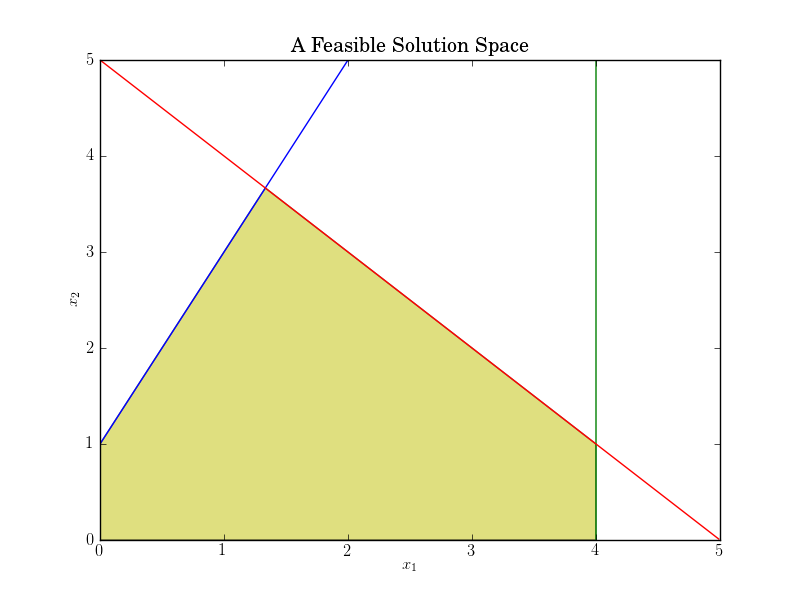
\includegraphics[height=7.5cm]{./backmatter/figs/feasible.png}
  \caption{An example of a feasible solution space.}
  \label{fig:feasible}
  \end{center}
\end{figure}

The program can become infeasible by adjusting a constraint. Take for instance,
an increased boundary constraint for $x_2$.

%%% 
\begin{subequations}\label{eqs:infeas}
  \begin{align}
    %%
    \max \:\: & 
    3 x_1 + 2 x_2
    & \label{eqs:infeas_obj} \\
    %%
    \text{s.t.} \:\: &
    -2 x_1 + x_2 \leq 1 \\
    %%
    &
    x_1 + x_2 \leq 5 
    & \label{eqs:infeas_sup} \\
    %%
    &
    x_1 \in [0, 4]
    &\label{eqs:infeas_x1} \\
    %%
    &
    x_2 \geq 4
    &\label{eqs:infeas_x2}
    %%
  \end{align}
\end{subequations}
%%% 

This arrangement results in the infeasible linear program shown in
Figure \ref{fig:infeasible}, where the updated constraint's effect is shown in
red.

\begin{figure}[H]
  \begin{center}
    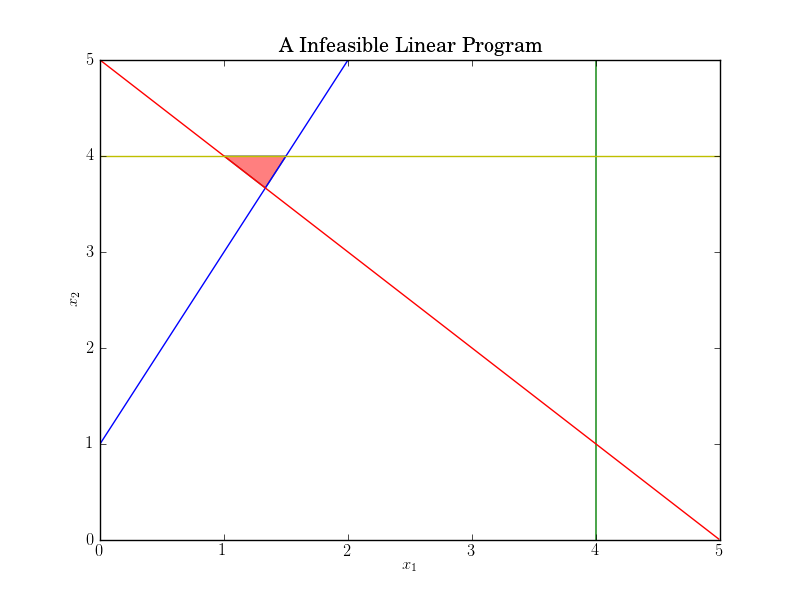
\includegraphics[height=7.5cm]{./backmatter/figs/infeasible.png}
  \caption{An example of a infeasible solution space.}
  \label{fig:infeasible}
  \end{center}
\end{figure}

The standard form of a linear program shown in Equation \ref{eqs:std-form} is an
example of a \textit{primal} linear program. A distinction is made between a
primal linear program and its \textit{dual}. Duality theory is involved and only
treated lightly in this review. The standard form of the dual of Equation
\ref{eqs:std-form} is given in Equation \ref{eqs:dual-form}.

%%% 
\begin{subequations}\label{eqs:dual-form}
  \begin{align}
    %%
    \max_{u} \:\: & 
    w = b^{\top} u
    & \label{eqs:dual-form_obj} \\
    %%
    \text{s.t.} \:\: &
    A^{\top} u \leq c 
    & \label{eqs:dual-form_sup} \\
    %%
    &
    u \geq 0
    &\label{eqs:dual-form_x}
    %%
  \end{align}
\end{subequations}
%%% 

A few critical differences exist. First note that the objective directions are
switched: if a primal form has a minimization objective, its dual has a
maximization objective. The constraint matrix is now $m \times n$-dimensional
(it is in fact the original constraint matrix transposed). There is a new series
of decision variables that form the corresponding solution space, i.e., the
positive vector $u$, as shown in Equation \ref{eqs:dual-form_obj}. These
variables are related to the original right-hand side of the constraint
formulation, the vector $b$. The costs of the original problem, $c$, now form
the right-hand side of the dual's constraint formulation,
Equation \ref{eqs:dual-form_sup}.

The concept of duality is critical in the field of mathematical programming
because it provides well-defined optimality characteristics of a given
program. These are achieved via the \textit{Strong Duality Theorem}
and \textit{Weak Duality Theorem}, shown below as stated
in \cite{ferris_linear_2008}.

\begin{thm}[Weak Duality Theorem]
If $x$ is primal feasible and $u$ is dual feasible, then the dual objective
function evaluated at $u$ is less than or equal to the primal objective function
at $x$.
\end{thm}

The Weak Duality Theorem provides inextricable linkage between a primal feasible
solution and dual feasible solution. If a dual feasible solution is found, it
provides a lower bound on the optimal solution. If a primal feasible solution is
found, it provides an upper bound on the optimal solution. Both of these
criteria, in tandem, help to greatly reduce the required search space during
optimization sweeps.

\begin{thm}[Strong Duality Theorem]
Exactly one of the following three alternatives hold:
\begin{enumerate}

  \item Both primal and dual problems are feasible and consequently both have
  optimal solutions with \textit{equal} extrema

  \item \textit{Exactly one} of the problems is infeasible and consequently the
  other problem has and unbounded objective function in the direction of
  optimization on its feasible region

  \item \textit{Both} primal and dual problems are infeasible

\end{enumerate}
\end{thm}

The Strong Duality Theorem provides the backbone for much of linear programming
theory and application. It states that not only do feasible solutions to the
primal and dual programs provide upper and lower bounds on optimal values, but
that, in fact, the optimal values are \textit{equal}. This provides a criterion
to \textit{know} when an optimal value is reached.

With this slight overview of the realm of linear programming, one can move on to
solution techniques for problems that can be represented as linear programs.

\section{The Simplex Method}

The Simplex Method is a popular algorithm to solve linear programs first
published by Dantzig \cite{dantzig_maximization_1951}. Conceptually, it is quite
intuitive, especially from a geometrical point of view. Before continuing in
more detail, an overview of the method is provided via the example from the
previous section. 

Note that there are five vertices of the polygon (i.e., a polytope more
generally) formed by the full set of constraints:

\begin{enumerate}
  \item $(0, 0)$
  \item $(0, 1)$
  \item $(\frac{4}{3}, \frac{11}{3})$
  \item $(4, 1)$
  \item $(4, 0)$
\end{enumerate}

The Simplex Method begins at a vertex, for example $(0, 0)$, and evaluates the
objective function.

\begin{equation}
    f(0, 0) = 3 * 0 + 2 * 0 = 0 
\end{equation}

Neighbor vertices are then evaluated, in order to determine which provides the
larger value (in the case of maximizing objectives).

\begin{equation}
    f(0, 1) = 3 * 0 + 2 * 1 = 2 
\end{equation}

\begin{equation}
    f(4, 0) = 3 * 4 + 2 * 0 = 12 
\end{equation}

The vertex $(4, 0)$ provides a larger objective function value, so the algorithm
moves to this vertex and determines the next largest neighbor. In this simple
example, there is only one choice, and it is trivially larger.

\begin{equation}
    f(4, 1) = 3 * 4 + 2 * 1 = 14 
\end{equation}

Accordingly the algorithm moves a second time, analyzing the neighboring
vertices again.

\begin{equation}
    f(\frac{4}{3}, \frac{11}{3}) = 3 * \frac{4}{3} + 2 * \frac{11}{3} = \frac{34}{3} 
\end{equation}

At this last move, a terminating condition has been achieved: a vertex has been
found for which all of its neighbors provide a lower value for the objective
function, i.e.,

\begin{equation}
    14 \geq 12 \:\:\: \text{and} \:\:\: 14 \geq \frac{34}{3}.
\end{equation}

Thus, the optimal value for $(x_1, x_2)$ has been determined to be $(4, 1)$. It
is immediately obvious that the simplex algorithm in this state is a hill
climbing (or hill descending) algorithm. The chief reason why this is possible
(i.e., why one is guaranteed to find a globally optimum solution) is that the
objective function and constraints are \textit{convex} functions of the decision
variables. Convexification is required to find optimum solutions to both linear
and integer programs.

In general, the Simplex Method is efficient, i.e., for most cases solutions are
found in less than exponential time in the number of variables. There are
certain program structures for which solution times are exponential, however,
and it in such cases, more advanced \textit{Interior Point} techniques are
required. In general, Interior Point algorithms are often much faster than
Simplex Algorithms \cite{ferris_linear_2008}, but are beyond the scope of this
review.

To begin a more robust discussion of the Simplex Method, one must introduce the
notion of \textit{slack variables}. Slack variables are used to transform
inequality constraints into equality constraints, effectively taking the
``slack'' out of the system. Slack variables are always positive, thus one could
use a slack variable, $s$, to convert

\begin{equation}
  \sum_{i} a_i x_i \leq b
\end{equation}

to 

\begin{equation}
  \sum_{i} a_i x_i + s = b
\end{equation}

and

\begin{equation}
  \sum_{i} a_i x_i \geq b
\end{equation}

to 

\begin{equation}
  \sum_{i} a_i x_i - s = b.
\end{equation}

The addition of slack variables allows one to rewrite an LP given in the
standard form of Equation \ref{eqs:std-form} as the \textit{canonical form}.

%%% 
\begin{subequations}\label{eqs:can-form}
  \begin{align}
    %%
    \min_{x, s} \:\: & 
    z =  c^{\top} x + 0^{\top} s
    & \label{eqs:can-form_obj} \\
    %%
    \text{s.t.} \:\: &
    A x - b = s
    & \label{eqs:can-form_sup} \\
    %%
    &
    x, s \geq 0
    &\label{eqs:can-form_x}
    %%
  \end{align}
\end{subequations}
%%% 

Given that there are $N$ decision variables and $M$ constraints, the cardinality
of $x$ is $N$ and the cardinality of $s$ is $M$. Furthermore, in the literature,
the $x_i$ variables are termed \textit{nonbasic} variables whereas the $s_i$
variables are termed \textit{basic} variables.

For any LP in the canonical form, the Simplex Algorithm can be applied to it to
determine optimal values for its decision variables, or to determine that it is
unbounded or infeasible. The basic structure of the method is outlined below in
Algorithm \ref{alg:simplex}.

\begin{algorithm}[h!]
 \SetAlgoLined
 \KwData{Decision variables, an objective function, and a set of constraints.}
 \KwResult{Optimal values for the decision variables or a flag denoting 
   infeasibility or unboundedness.}
 Get initial vertex\;
 \If{no vertex is found}{
 feasible solution space is empty\;
 }
 \While{not unbounded and not empty and not done}{ 
    Select column, i, via pricing\;
    \If{no column is found}{
    optimal condition found\;
    done\;
    }
    Select row, j, via the ratio test\;
    \If{no row is found}{
    solution space is unbounded\;
    }
    Perform a Jordan exchange on element (i, j)\;
  }
  \caption{The Simplex Algorithm}\label{alg:simplex}
\end{algorithm}

There are four core operations associated with the Simplex Algorithm:
\begin{enumerate}
  \item finding an initial vertex
  \item column pricing
  \item row selection
  \item exchanging elements
\end{enumerate}

If finding an initial vertex is not trivial (e.g., if the origin is not a
candidate), then the operation to do so requires use of the Simplex Method on a
related LP where the origin is an available candidate. That process will be
described last.

The primary concept required to understand the Simplex Method's operations is
that of the \textit{basis}. The basis begins as the set of decision
variables. The algorithm progresses by moving slack variables into the basis,
and it does so efficiently by analyzing the most ``valuable'' variables to
target (i.e., which current basis variable affects the optimal value the most).

Column pricing and row selection are the operations that select the current
basis and nonbasis variables to target. The Jordan exchange process translates
the formulation into the new basis, exchanging basic and nonbasic
variables. This is perhaps more intuitive from a geometrical point of
view. Consider some starting vertex with many possible sides along which to
move. The process of column pricing and row selection \textit{chooses} the side
along which to move, and the Jordan exchange \textit{reorients} the
problem. Revisiting the example problem, remember the first step. The vertex
$(4, 0)$ was determined to be the best direction in which to move. After a
Jordan exchange, the resulting LP would look like Figure \ref{fig:rotated}.

\begin{figure}[H]
  \begin{center}
    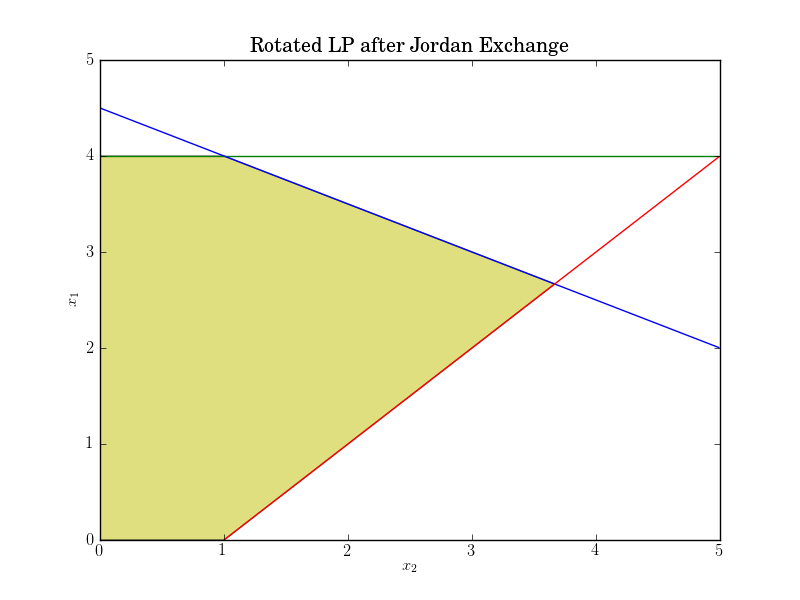
\includegraphics[height=7.5cm]{./backmatter/figs/rotated.png}
  \caption{The Reoriented LP after the first Jordan Exchange.}
  \label{fig:rotated}
  \end{center}
\end{figure}

The column pricing operation selects the slack variable which will enter the
basis. The most naive implementation is to select the variable which will have
the largest effect on the objective function, i.e., which has the largest
magnitude \textit{reduced cost}. For instance, in Equation \ref{eqs:lp_obj},
$x_1$ has a reduced cost of 3, and $x_2$ has a reduced cost of 2 (note that both
costs are in the same positive direction as the objective, i.e.,
maximization). Accordingly, choosing $x_1$ as the nonbasic exchange variable is
a valid option. However, any algorithm may be used to make this selection, as
long as the reduced cost is positive.

Row selection, i.e., selecting the basic variable to enter the basis, is
performed via a ratio test. Given that a column $j$ has been selected, the
corresponding row is selected according to Equation \ref{eqs:ratio-max} in the
case of a maximization objective and Equation \ref{eqs:ratio-min} in the case of
a minimization objective.

\begin{equation}\label{eqs:ratio-max}
  \min \left\{ \frac{-b_i}{A_{i,j}} \:\: | \:\: A_{i,j} > 0 \right\}
\end{equation}

\begin{equation}\label{eqs:ratio-min}
  \min \left\{ \frac{-b_i}{A_{i,j}} \:\: | \:\: A_{i,j} < 0 \right\}
\end{equation}

The Jordan Exchange operation, which transforms a matrix $A \mapsto A'$
given a pivot $(\hat{\imath}, \hat{\jmath})$, is straightforward and is shown in
Equation \ref{eqs:jordan}.

%%% 
\begin{subequations}\label{eqs:jordan}
  \begin{align}
    %%
    a_{\hat{\imath},\hat{\jmath}}' = \frac{1}{a_{\hat{\imath},\hat{\jmath}}}
    &\:\: \text{for} \:
    i = \hat{\imath}, j = \hat{\jmath} \\
    %%
    a_{\hat{\imath},j}' = -\frac{a_{\hat{\imath},j}}{a_{\hat{\imath},\hat{\jmath}}}
    &\:\: \text{for} \:
    i = \hat{\imath}, j \neq \hat{\jmath} \\
    %%
    a_{i,\hat{\jmath}}' = \frac{a_{i,\hat{\jmath}}}{a_{\hat{\imath},\hat{\jmath}}}
    &\:\: \text{for} \:
    i \neq i, j = \hat{\jmath} \\
    %%
    a_{i,j}' = a_{i,j} - a_{i,\hat{\jmath}} a_{\hat{\imath},j}
    &\:\: \text{for} \:
    i \neq \hat{\imath}, j \neq \hat{\jmath}
    %%
  \end{align}
\end{subequations}
%%% 

Finally, one must determine a starting vertex. The original linear program is
modified as shown in \S 3.4 of \cite{ferris_linear_2008}. For each row, $i$, if
$b_i > 0$, then add an additional variable, $x_0$, to the constraint with
coefficient $a_{i,0} = 1$. An initial feasible point is then immediately
available for $x = 0 \:\: \forall \:\: i \neq 0$ and $x_0
= \max(\max(b),0)$. The Simplex Method is then applied, with $x_0$ being the
first variable to leave the basis. When $x_0$ returns to the basis, a suitable
starting vertex results from the removal of $x_0$.

\chapter{Integer Programming and the Branch-And-Bound Method}\label{app:ip}

Integer programming expands upon the possible problems that can be modeled by
linear programming. Decision variables in linear programming are optimized on a
continuum, i.e., all decision variables, $x$, are real numbers,
$x \in \mathbb{R}^n$. Integer programming allows for certain decision variables,
$y$, to take on integer-only values, i.e., $y \in \mathbb{Z}^n$. Strictly
speaking, a programming formulation for which all decision variables are integer
(i.e., integer and binary) is called an \textit{integer program} (IP), whereas a
programming formulation for which some decision variables are integer while
others are linear is called a \textit{mixed integer-linear program} (MILP). The
discussion that follows is informed largely by Wolsey's
text \cite{wolsey_integer_1998} from which I cite many definitions,
etc. Additional clarification comes from course notes \cite{luedtke_class_2010}.

\section{Integer Programming}

Integer programming allows one to model specialized decision cases. Take for
example one of the most well-known problems in mathematical programming and
optimization, the \textit{Knapsack Problem}. A version of the Knapsack problem
is described as follows:

\begin{itemize}
        \item A knapsack can hold at most $b$ pounds. 
        \item There are $n$ possible items that can be placed in the bag.
        \item Each item is characterized by a preference, or benefit, $c_i$, 
              and a weight, $a_i$
        \item One would like to maximize the benefit associated with a knapsack
\end{itemize}

The decision variables, $y_i$s, for the Knapsack Problem provide its integer
nature. Any given item in the above formulation can only be added once. Indeed,
consider that for any viable solution, each item is in one of two distinct
states: included in the knapsack or excluded from the knapsack. This duality of
states provides a natural usage of binary variables, i.e., a variable that has
only two states, 0 and 1. Accordingly, the Knapsack Problem as an integer
program is formulated as Equation \ref{eqs:knapsack}.

%%% 
\begin{subequations}\label{eqs:knapsack}
  \begin{align}
    %%
    \max \:\: & 
    \sum_{i \in I} c_i y_i
    & \\
    %%
    \text{s.t.} \:\: &
    \sum_{i \in I} a_i y_i \leq b 
    & \\
    %%
    &
    y_i \in \{ 0, 1 \}
    &
    \forall i \in I
    %%
  \end{align}
\end{subequations}
%%% 

Optimization problems are given as formulations, a series of inequality
equations. Both domain knowledge and geometrical investigation can provide
better formulations than may be evident from an initial formulation. Formally, a
formulation forms a polyhedron.

\begin{define}\label{def:polyhedron}
A subset of $\mathbb{R}^n$ described by a finite set of linear constraints $P
= \{ x \in \mathbb{R}^n : Ax \leq b\}$ is a \textbf{polyhedron}.
\end{define}

\begin{define}\label{def:formulation}
A polyhedron $P \subseteq \mathbb{R}^{n+p}$ is a \textbf{formulation} for a set
$X \subseteq \mathbb{Z}^n \times \mathbb{R}^p$ iff $X = P \cap \left( 
\mathbb{Z}^n \times \mathbb{R}^p \right)$
\end{define}

As previously noted, more than one formulation can be viable for a given
problem. Let us return to the Knapsack Problem in
Equation \ref{eqs:knapsack}. Consider a knapsack with $b = 5$ and items with
$a_1 = 2$, $a_2 = 3$, $a_3 = 4$. The original formulation is as follows.

%%% 
\begin{subequations}\label{eqs:knapsack1}
  \begin{align}
    %%
    \max \:\: & 
    \sum_{i \in I} c_i y_i
    & \\
    %%
    \text{s.t.} \:\: &
    2y_1 + 3y_2 + 4y_3 \leq 5 
    & \\
    %%
    &
    y_i \in \{ 0, 1 \}
    &
    \forall i \in I
    %%
  \end{align}
\end{subequations}
%%% 

The set of feasible solutions here forms a polyhedron from the points $Y = {(0,
0, 0), (1, 0, 0), (0, 1, 0), (0, 0, 1), (1, 1, 0)}$. The optimal solution will
depend on values given to each item's benefit, $c_i$. However, the formulation
as provided defines a solution space larger than the specific points mentioned
here. One could add a constraint, say, 

\begin{equation}
y_1 + y_3 \leq 1
\end{equation}

or 

\begin{equation}
y_2 + y_3 \leq 1.
\end{equation}

These two derived constraints state that the third item, if chosen, can not be
included with either the first or the second item. The resulting formulation is
shown in Equation \ref{eqs:knapsack2}.

%%% 
\begin{subequations}\label{eqs:knapsack2}
  \begin{align}
    %%
    \max \:\: & 
    \sum_{i \in I} c_i y_i
    & \\
    %%
    \text{s.t.} \:\: &
    2y_1 + 3y_2 + 4y_3 \leq 5 
    & \\
    %%
    &
    y_1 + y_3 \leq 1        
    & \\
    %%
    &
    y_2 + y_3 \leq 1        
    & \\
    %%
    &
    y_i \in \{ 0, 1 \}
    &
    \forall i \in I
    %%
  \end{align}
\end{subequations}
%%% 

It is obvious that Equation \ref{eqs:knapsack2} is a different formulation than
Equation \ref{eqs:knapsack1}. For example, the point $(0.9, 0.5, 0.4)$ resides
in the feasible solution space of Equation \ref{eqs:knapsack1} but is outside of
the feasible solution space of Equation \ref{eqs:knapsack2}. Intuitively, a
smaller solution space can be searched more quickly, thus \textit{tighter}
formulations require less time to solve in general.

The notion of one formulation being ``better'' than another can be formally
expressed.

\begin{define}
Given a feasible solution space set $X \subseteq \mathbb{R}^n$ and two
formulations, $P_1$ and $P_2$, for $X$, $P_1$ is a \textbf{better formulation}
than $P_2$ if $P_1 \subset P_2$.
\end{define}

There is, of course, a limit to the formulations one can develop for a given
problem. A fully-restricted solution space, i.e., one that is as tightly bounded
as possible, is called the problem's \textit{convex hull}. 

\begin{define}
Given a set $X \subseteq \mathbb{R}^n$, the \textbf{convex hull} of $X$, denoted
$conv(X)$, is defined as: $conv(X) = \{x : x = \sum_{i=1}^{t} \lambda_i
x_i, \sum_{i=1}^{t} \lambda_i = 1, \lambda_i \geq 0$ for $i = 1, \ldots, t$ over
all finite subsets $\{x^1, \ldots, x^t \}$ of $X\}$.
\end{define}

Because the extreme points of $conv(X)$ all lie in $X$, the equivalent LP can be
used instead of the IP. Convex hull formulations are rarely seen in practice,
however, because they require an exponential number of additional
constraints \cite{wolsey_integer_1998}. While the convex hull of a given problem
may not be discovered in practice, the feasible solution space most assuredly is
reduced by most solution techniques. From a geometrical point of view, this acts
as cutting off solution space from some original larger space through the
addition of constraints as shown above. Accordingly, these additional
constraints are termed \textit{cutting planes}.

\section{The Branch and Bound Algorithm}\label{sec:bnb}

One of the most popular solution techniques used to solve integer programs is an
algorithm called \textit{Branch and Bound} (BNB). At its core, BNB is a
divide-and-conquer search algorithm that uses an enumeration tree to find
optimal solutions to $\mathcal{NP}$-hard IPs and MILPs. There are a number of
ways to speed up the search based on general techniques and problem-specific
insights, a number of which have been discussed in the previous section. This
section highlights the basic nature of the algorithm and discusses lightly some
of the variety of solution strategies available. Again, the discussion here
comes largely from \cite{wolsey_integer_1998} and \cite{luedtke_class_2010}.

BNB utilizes the \textit{relaxation} of a given IP or MILP. A relaxation is a
related reformulation of a given problem that is generally easier to solve. In
the case of a linear programming relaxation, integer variables in the IP or MILP
are relaxed and allowed to be linear variables. Solving this formulation is
advantageous because it provides an \textit{upper bound} for the IP or
MILP. Similarly, solving a dual, given that it is feasible and has a finite
solution, or using some other heuristic provides a \textit{lower bound}. These
bounds allow the search tree to terminate, or \textit{prune}, a
given \textit{branch}.

A simple example greatly helps to show the process of the BNB algorithm. Let us
use a specific instance of Equation \ref{eqs:knapsack}. This example is
contrite and does not involve pruning; it is useful simply to show how
branching occurs. Consider a knapsack with three items. The items have benefits
of 0.5, 1, and 1.4, respectively and weights of 2, 3, and 4 pounds,
respectively. The knapsack can hold 5 pounds. The integer program is shown in
Equation \ref{eqs:knapsack-ip} and the LP relaxation is shown in
Equation \ref{eqs:knapsack-lp}.

%%% 
\begin{subequations}\label{eqs:knapsack-ip}
  \begin{align}
    %%
    \max \:\: & 
    Z^{IP} = 0.5 y_1 + y_2 + 1.4 y_3
    & \\
    %%
    \text{s.t.} \:\: &
    2y_1 + 3y_2 + 4y_3 \leq 5 
    & \\
    %%
    &
    y_1, y_2, y_3 \in \{ 0, 1 \}
    %%
  \end{align}
\end{subequations}
%%% 

%%% 
\begin{subequations}\label{eqs:knapsack-lp}
  \begin{align}
    %%
    \max \:\: & 
    Z^{LP} = 0.5 y_1 + y_2 + 1.4 y_3
    & \\
    %%
    \text{s.t.} \:\: &
    2y_1 + 3y_2 + 4y_3 \leq 5 
    & \\
    %%
    &
    y_1, y_2, y_3 \in [0, 1]
    %%
  \end{align}
\end{subequations}
%%% 

Solving the relaxation provides an upper bound of $Z^{LP} = \frac{26}{15}$, a
(non-integer) solution of $y' = (0, \frac{1}{3}, 1)$ and a root node for the BNB
search tree, shown in Figure \ref{fig:root}.

\begin{figure}[H]
  \begin{center}
    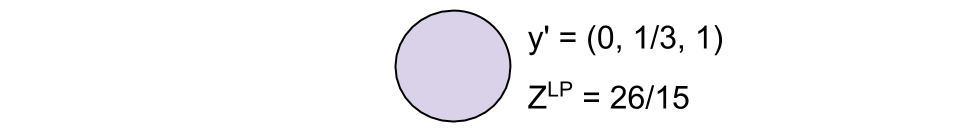
\includegraphics[width=0.8\linewidth]{./backmatter/figs/root.png}
  \caption{The root node for the BNB algorithm associated with 
  Equation \ref{eqs:knapsack-ip}.}
  \label{fig:root}
  \end{center}
\end{figure}

The algorithm then chooses a variable on which to \textit{branch}. Formally
branching divides the set of feasible solution spaces in two. Given a solution
space $S$, branching on a binary variable $y_i$, produces two new solution
spaces.

\begin{equation}
\begin{split}
& S_1 = S \cap \{y: y_i = 0\}
\\
& S_2 = S \cap \{y: y_i = 1\}
\end{split}
\end{equation}

If the variable is non-binary integer, given a non-integer feasible solution,
$y'$, one produces the following new spaces.

\begin{equation}
\begin{split}
& S_1 = S \cap \{y: y_i \leq \lfloor y_i' \rfloor\}
\\
& S_2 = S \cap \{y: y_i \geq \lceil y_i' \rceil\}
\end{split}
\end{equation}

Arbitrarily, for this example case, one could choose to branch on
$y_2$. The resulting relaxations are shown as Equation \ref{eqs:y2-0} for $y_2 =
0$ and Equation \ref{eqs:y2-1} for $y_2 = 1$.

%%% 
\begin{subequations}\label{eqs:y2-0}
  \begin{align}
    %%
    \max \:\: & 
    Z^{LP} = 0.5 y_1 + 1.4 y_3
    & \\
    %%
    \text{s.t.} \:\: &
    2 y_1 + 4 y_3 \leq 5 
    & \\
    %%
    &
    y_1, y_3 \in [0, 1]
    %%
  \end{align}
\end{subequations}
%%% 

%%% 
\begin{subequations}\label{eqs:y2-1}
  \begin{align}
    %%
    \max \:\: & 
    Z^{LP} = 0.5 y_1 + 1 + 1.4 y_3
    & \\
    %%
    \text{s.t.} \:\: &
    2 y_1 + 3 + 4 y_3 \leq 5 
    & \\
    %%
    &
    y_1, y_3 \in [0, 1]
    %%
  \end{align}
\end{subequations}
%%% 

Each of these new subproblems become \textit{active nodes} and are added to
the \textit{active list}. Active nodes are subproblem nodes that have been
recognized by the algorithm and the next subproblem to solve is chosen from the
active list by some strategy. For this simple case, both subproblems are solved
and the resulting values are shown in Figure \ref{fig:branch}.

\begin{figure}[H]
  \begin{center}
    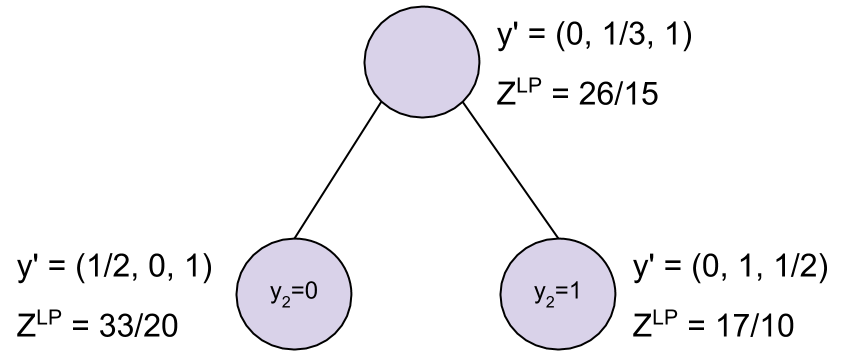
\includegraphics[height=5.5cm]{./backmatter/figs/branch.png}
  \caption{The first two branches of the BNB algorithm associated with 
  Equations \ref{eqs:y2-0} and \ref{eqs:y2-1}.}
  \label{fig:branch}
  \end{center}
\end{figure}

One could continue in this manner, branching on subsequent variables and
enumerating all possible solutions, to eventually reach the optimal solution of
$y^* = (1, 1, 0)$. However, so far we have ignored pruning, the act of
terminating a branch of the search tree, knowing that no further useful
information can be gained from its investigation. Pruning provides the
``bounding'' aspect of the Branch and Bound algorithm.

At any point in the process of the BNB algorithm, there is a known global upper
bound, $U$, to the optimal solution and lower bound, $L$, to the optimal
solution. Accordingly, a branch of the enumeration search tree can be pruned in
three instances:

\begin{enumerate}
        \item The subproblem is optimal, given its subspace of the feasible
        option space.
        \item The subproblem has a known upper bound that is lower
        than the global lower bound or the subproblem has a known lower bound
        that is larger than the global upper bound.
        \item The subproblem is infeasible.
\end{enumerate}

With the above background, the actual BNB algorithm can be presented.
\\
\begin{algorithm}[H]
 \SetAlgoLined
 \KwData{Decision variables, an objective function, and a set of constraints.}
 \KwResult{Optimal values for the decision variables or a flag denoting 
   infeasibility or unboundedness.}
 Perform any \emph{preprocessing operations}\;
 Derive a lower bound, $L$, via a \emph{heuristic}\;
 Place original problem on the active list\;
 \While{The active list is \textit{not} empty}{
       Use a \emph{strategy} to select a candidate node ($S$) from the active 
       list\;
       Solve the LP relaxation to get an upper bound for the candidate, $U(S)$\;
       \If{$U(S) > U$}{$U \leftarrow U(S)$\;}
       \If{$S$ is infeasible}{
           prune the branch\;
       }
       \ElseIf{$U(S) > L$}{
           $L \leftarrow U(S)$\;
       }
       \ElseIf{$U(S) < L$}{
           prune the branch\;
       }
       \Else{
           branch on $S$\;
           add new subproblems to the active list\;
       }           
       Remove $S$ from the active list\;
 }
 \caption{The Branch and Bound Algorithm}
\end{algorithm}

There are three ways to assist, or speed up, the Branch and Bound algorithm as
highlighted above:
\begin{enumerate}
        \item Preprocessing
        \item Lower-bound heuristics
        \item Node selection strategies
\end{enumerate}

Preprocessing is a step provided by many solvers. It generally involves an
investigation of the problem instance in order to minimize future
work. Preprocessing can affect solution bounds by tightening bounds or providing
cutoffs to the solver (i.e., preformed feasible solutions). It can speed up the
internal Simplex Method processing by informing the solver as to good simplex
pricing strategies. The feasible solution space can also be reduced by finding
redundant constraints and providing cutting planes, as discussed in the previous
section. Finally, the preprocessing step can \textit{a priori} fix certain
decision variables. The variable fixing algorithm is straightforward.

\begin{algorithm}[H]
 \SetAlgoLined
 \KwData{An constraint matrix, $A$, objective coefficients, $c$, and decision 
 variables $x$ with decision variable lower bounds, $l$, and upper bounds 
 $u$.}
 \KwResult{A (possibly empty) set of fixed variables.}
 \ForEach{decision variable, $x_j$,}{
   \If{$a_{i,j} \geq 0 \;\; \forall \;\; i$ {\emph{and}} $c_j < 0$}{
     $x_j \leftarrow l_j$\;
   }
   \ElseIf{$a_{i,j} \leq 0 \;\; \forall \;\; i$ {\emph{and}} $c_j > 0$}{
     $x_j \leftarrow u_j$\;
   }       
 }  
 \caption{The Variable Fixing Algorithm for a Maximization Objective Function}
\end{algorithm}

A variety of lower-bound heuristics exist. Some of the most popular involve
solving heavily restricted versions of the original problem or diving down the
enumeration tree, rounding fractional integer values. There are also
problem-specific heuristics that depend on well-known problem structures.

Finally, there exist nominally three well-used node selection strategies. The
first is called the \textit{Best Node Search} (BNS) which chooses the next best
node in the active list based based on the node's upper bound. This requires
large movement around the search tree, effectively solving dissimilar
relaxations. The second is the well-known \textit{Depth First Search} (DFS). A
DFS for an IP-enumeration tree is beneficial because subsequent relaxations are
related, which allows for \textit{warm start} of the LP relaxations. Warm starts
allow subsequent relaxations to be solved quickly because good approximations to
the optimal solution can be provided. The final strategy is a \textit{BNS-DFS
hybrid}. The hybrid strategy involves estimating an optimal value, performing a
DFS until the relaxation's optimal value is below that of the estimation, and
then choosing the next-best node to continue.

\chapter{Cyclopts HDF5 Database Layout}\label{app:hdf5}

This appendix details the exact database layout used by Cyclopts for the
ExchangeFamily, StructuredRequest species, and StructuredSupply species.

\section{Parameter Space}

Both front-end and back-end species record the state of every point in a given
parameter space in a data set called \code{/Species/<species type>/Points},
where \code{<species type>} is either \code{StructuredRequest} or
\code{StructuredSupply}. Each point incorporates both fundamental and instance
parameters as described in \S \ref{method:setup}. The tables associated with
parameter spaces are described below.

\begin{table}[h!]
\centering
\label{tbl:/Species/StructuredRequest/Points}
\caption{Datatype description of the \lstinline[basicstyle=\ttfamily\color{black}]|/Species/StructuredRequest/Points| dataset.}
\begin{tabularx}{\columnwidth-10pt}{|c|c|X|} % line wraps second column if too long
\hline
\textbf{Name} & \textbf{Data Type} & \textbf{Description}       \\ \hline
paramid & 16-character string & The hex value of a UUID for a point in parameter space. \\ \hline
family & 30-character string & A description of the problem family \\ \hline
f\_fc & 1-byte integer & As described in \S \ref{method:setup} \\ \hline
f\_loc & 1-byte integer & As described in \S \ref{method:setup} \\ \hline
f\_mox & 4-byte float & As described in \S \ref{method:setup} \\ \hline
f\_rxtr & 1-byte integer & As described in \S \ref{method:setup} \\ \hline
n\_reg & 4-byte unsigned integer & As described in \S \ref{method:setup} \\ \hline
n\_rxtr & 4-byte unsigned integer & As described in \S \ref{method:setup} \\ \hline
r\_inv\_proc & 4-byte float & As described in \S \ref{method:setup} \\ \hline
r\_l\_c & 4-byte float & As described in \S \ref{method:setup} \\ \hline
r\_s\_mox & 4-byte float & As described in \S \ref{method:setup} \\ \hline
r\_s\_mox\_uox & 4-byte float & As described in \S \ref{method:setup} \\ \hline
r\_s\_th & 4-byte float & As described in \S \ref{method:setup} \\ \hline
r\_s\_thox & 4-byte float & As described in \S \ref{method:setup} \\ \hline
r\_t\_f & 4-byte float & As described in \S \ref{method:setup} \\ \hline
r\_th\_pu & 4-byte float & As described in \S \ref{method:setup} \\ \hline
seed & 8-byte integer & The random seed used to generate an instance. \\ \hline
\end{tabularx}
\end{table}


\begin{table}[h!]
\centering
\label{tbl:/Species/StructuredSupply/Points}
\caption{Datatype description of the \lstinline[basicstyle=\ttfamily\color{black}]|/Species/StructuredSupply/Points| dataset.}
\begin{tabularx}{\columnwidth-10pt}{|c|c|X|} % line wraps second column if too long
\hline
\textbf{Name} & \textbf{Data Type} & \textbf{Description}       \\ \hline
paramid & 16-character string & The hex value of a UUID for a point in parameter space. \\ \hline
family & 30-character string & A description of the problem family \\ \hline
d\_f\_mox & 4-length array of 8-byte floats & As described in \S \ref{method:setup} \\ \hline
d\_f\_thox & 4-length array of 8-byte floats & As described in \S \ref{method:setup} \\ \hline
d\_th & 3-length array of 8-byte floats & As described in \S \ref{method:setup} \\ \hline
f\_fc & 1-byte integer & As described in \S \ref{method:setup} \\ \hline
f\_loc & 1-byte integer & As described in \S \ref{method:setup} \\ \hline
f\_mox & 4-byte float & As described in \S \ref{method:setup} \\ \hline
f\_rxtr & 1-byte integer & As described in \S \ref{method:setup} \\ \hline
n\_reg & 4-byte unsigned integer & As described in \S \ref{method:setup} \\ \hline
n\_rxtr & 4-byte unsigned integer & As described in \S \ref{method:setup} \\ \hline
r\_inv\_proc & 4-byte float & As described in \S \ref{method:setup} \\ \hline
r\_l\_c & 4-byte float & As described in \S \ref{method:setup} \\ \hline
r\_repo & 4-byte float & As described in \S \ref{method:setup} \\ \hline
r\_s\_mox & 4-byte float & As described in \S \ref{method:setup} \\ \hline
r\_s\_mox\_uox & 4-byte float & As described in \S \ref{method:setup} \\ \hline
r\_s\_th & 4-byte float & As described in \S \ref{method:setup} \\ \hline
r\_s\_thox & 4-byte float & As described in \S \ref{method:setup} \\ \hline
r\_t\_f & 4-byte float & As described in \S \ref{method:setup} \\ \hline
r\_th\_pu & 4-byte float & As described in \S \ref{method:setup} \\ \hline
seed & 8-byte integer & The random seed used to generate an instance. \\ \hline
\end{tabularx}
\end{table}

\section{Problem Instances}

Problem instances are generated by problem species and are executed by problem
families. Accordingly, both species and families can record information about
instances. Front and back-end exchange species each record two types of
information: details about each arc in an instance and a summary of
species-specific information. The exchange family records information regarding
each of the entities that comprise an instance: nodes, groups of nodes (having
been translated from portfolios), and arcs. Further, aggregate summary
information is also recorded. 

\subsection{Exchange Family}

The exchange family records information regarding all major constructs in an
exchange: nodes, groups, and arcs. A summary table is written to
\code{/Family/ResourceExchange/ExchangeInstProperties}. Nodes and group data are
recorded in an aggregate dataset located at
\code{/Family/ResourceExchange/ExchangeNodes}; node group data is located at
\code{/Family/ResourceExchange/ExchangeGroups}; and arc data is collected in the
\code{/Family/ResourceExchange/ExchangeArcs} group. A dataset per instance UUID
is used because it has been found to be useful in the postprocessing phase. A
summary of family-specific instance data are detailed below.

\begin{table}[h!]
\centering
\label{tbl:/Family/ResourceExchange/ExchangeInstProperties}
\caption{Datatype description of the \lstinline[basicstyle=\ttfamily\color{black}]|/Family/ResourceExchange/ExchangeInstProperties| dataset.}
\begin{tabularx}{\columnwidth-10pt}{|c|c|X|} % line wraps second column if too long
\hline
\textbf{Name} & \textbf{Data Type} & \textbf{Description}       \\ \hline
paramid & 16-character string & The hex value of a UUID for a point in parameter space. \\ \hline
instid & 16-character string & The hex value of a UUID for an NFCTP graph instance. \\ \hline
species & 30-character string & A description of a problem species. \\ \hline
n\_arcs & 8-byte integer & The number of arcs in an NFCTP instance. \\ \hline
n\_u\_grps & 8-byte integer & The number of supply groups in an NFCTP instance. \\ \hline
n\_v\_grps & 8-byte integer & The number of demand groups in an NFCTP instance. \\ \hline
n\_u\_nodes & 8-byte integer & The number of supply nodes in an NFCTP instance. \\ \hline
n\_v\_nodes & 8-byte integer & The number of demand nodes in an NFCTP instance. \\ \hline
n\_constrs & 8-byte integer & The number of constraints in an NFCTP instance. \\ \hline
excl\_frac & 8-byte float & The fraction of arcs in a NFCTP graph that are exclusive. \\ \hline
\end{tabularx}
\end{table}

\begin{table}[h!]
\centering
\label{tbl:/Family/ResourceExchange/ExchangeNodes}
\caption{Datatype description of the \lstinline[basicstyle=\ttfamily\color{black}]|/Family/ResourceExchange/ExchangeNodes| dataset.}
\begin{tabularx}{\columnwidth-10pt}{|c|c|X|} % line wraps second column if too long
\hline
\textbf{Name} & \textbf{Data Type} & \textbf{Description}       \\ \hline
instid & 16-character string & The hex value of a UUID for an NFCTP graph instance. \\ \hline
id & 8-byte integer & A uniquely identifying value. \\ \hline
gid & 8-byte integer & A unique value identifying an ExchangeGroup \\ \hline
kind & 1-byte integer bitfield & Whether an object is associated with supply or demand. \\ \hline
qty & 8-byte float & A quantity. \\ \hline
excl & 1-byte integer bitfield & Whether or not an arc is exclusive. \\ \hline
excl\_id & 8-byte integer & A unique value identifying the mutually exclusive group an arc belongs to. \\ \hline
\end{tabularx}
\end{table}

\begin{table}[h!]
\centering
\label{tbl:/Family/ResourceExchange/ExchangeGroups}
\caption{Datatype description of the \lstinline[basicstyle=\ttfamily\color{black}]|/Family/ResourceExchange/ExchangeGroups| dataset.}
\begin{tabularx}{\columnwidth-10pt}{|c|c|X|} % line wraps second column if too long
\hline
\textbf{Name} & \textbf{Data Type} & \textbf{Description}       \\ \hline
instid & 16-character string & The hex value of a UUID for an NFCTP graph instance. \\ \hline
id & 8-byte integer & A uniquely identifying value. \\ \hline
kind & 1-byte integer bitfield & Whether an object is associated with supply or demand. \\ \hline
caps & 4-length array of 8-byte floats & Capacity RHS values. \\ \hline
cap\_dirs & 4-length array of 1-byte integer bitfields & Whether a constraint is greater or less-than \\ \hline
qty & 8-byte float & A quantity. \\ \hline
\end{tabularx}
\end{table}

\begin{table}[h!]
\centering
\label{tbl:/Family/ResourceExchange/ExchangeArcs/id_8017b48888ac424fb991527195a831b6}
\caption{Datatype description of the \lstinline[basicstyle=\ttfamily\color{black}]|/Family/ResourceExchange/ExchangeArcs/<Instance UUID>| dataset.}
\begin{tabularx}{\columnwidth-10pt}{|c|c|X|} % line wraps second column if too long
\hline
\textbf{Name} & \textbf{Data Type} & \textbf{Description}       \\ \hline
id & 8-byte integer & A uniquely identifying value. \\ \hline
uid & 8-byte integer & Supply node for an arc. \\ \hline
ucaps & 4-length array of 8-byte floats & Capacity coefficients for a supply node. \\ \hline
vid & 8-byte integer & Request node for an arc. \\ \hline
vcaps & 4-length array of 8-byte floats & Capacity coefficients for a request node. \\ \hline
pref & 8-byte float & Preference value of an arc. \\ \hline
\end{tabularx}
\end{table}

\subsection{Exchange Species}

Both exchange species record information about each arc in an exchange
instance. A parent group for arc data is defined under each species group. A
group for each instance, whose name is the hex string of the UUID, is defined
under the associated arc group. Finally, arc information associated with each
instance is stored as a dataset in that instance's group. For example, the arc
data for a given UUID of a front-end exchange is located as a dataset in the
group \code{/Species/StructuredRequest/Arcs/<UUID hex>}. Summary information
related to each species is also recorded in a data set for each species type
located in the group \code{/Species/<species type>/Summary}. Tables describing
species-specific instance data are detailed below.

\begin{table}[h!]
\centering
\label{tbl:/Species/StructuredRequest/Arcs/id_8017b48888ac424fb991527195a831b6}
\caption{Datatype description of the \lstinline[basicstyle=\ttfamily\color{black}]|/Species/<Species Type>/Arcs/<Instance UUID>| dataset.}
\begin{tabularx}{\columnwidth-10pt}{|c|c|X|} % line wraps second column if too long
\hline
\textbf{Name} & \textbf{Data Type} & \textbf{Description}       \\ \hline
arcid & 4-byte unsigned integer & The hex value of a UUID for an arc. \\ \hline
commod & 4-byte unsigned integer & The commodity associated with an arc. \\ \hline
pref\_c & 4-byte float & Commodity-based preference of an arc. \\ \hline
pref\_l & 4-byte float & Location-based preference of an arc. \\ \hline
\end{tabularx}
\end{table}

\begin{table}[h!]
\centering
\label{tbl:/Species/StructuredRequest/Summary}
\caption{Datatype description of the \lstinline[basicstyle=\ttfamily\color{black}]|/Species/StructuredRequest/Summary| dataset.}
\begin{tabularx}{\columnwidth-10pt}{|c|c|X|} % line wraps second column if too long
\hline
\textbf{Name} & \textbf{Data Type} & \textbf{Description}       \\ \hline
paramid & 16-character string & The hex value of a UUID for a point in parameter space. \\ \hline
family & 30-character string & A description of the problem family \\ \hline
n\_r\_th & 4-byte unsigned integer & As described in \S \ref{method:setup} \\ \hline
n\_r\_f\_mox & 4-byte unsigned integer & As described in \S \ref{method:setup} \\ \hline
n\_r\_f\_thox & 4-byte unsigned integer & As described in \S \ref{method:setup} \\ \hline
n\_s\_uox & 4-byte unsigned integer & As described in \S \ref{method:setup} \\ \hline
n\_s\_th\_mox & 4-byte unsigned integer & As described in \S \ref{method:setup} \\ \hline
n\_s\_f\_mox & 4-byte unsigned integer & As described in \S \ref{method:setup} \\ \hline
n\_s\_f\_thox & 4-byte unsigned integer & As described in \S \ref{method:setup} \\ \hline
\end{tabularx}
\end{table}

\begin{table}[h!]
\centering
\label{tbl:/Species/StructuredSupply/Summary}
\caption{Datatype description of the \lstinline[basicstyle=\ttfamily\color{black}]|/Species/StructuredSupply/Summary| dataset.}
\begin{tabularx}{\columnwidth-10pt}{|c|c|X|} % line wraps second column if too long
\hline
\textbf{Name} & \textbf{Data Type} & \textbf{Description}       \\ \hline
paramid & 16-character string & The hex value of a UUID for a point in parameter space. \\ \hline
family & 30-character string & A description of the problem family \\ \hline
n\_r\_th & 4-byte unsigned integer & As described in \S \ref{method:setup} \\ \hline
n\_r\_f\_mox & 4-byte unsigned integer & As described in \S \ref{method:setup} \\ \hline
n\_r\_f\_thox & 4-byte unsigned integer & As described in \S \ref{method:setup} \\ \hline
n\_s\_uox & 4-byte unsigned integer & As described in \S \ref{method:setup} \\ \hline
n\_s\_th\_mox & 4-byte unsigned integer & As described in \S \ref{method:setup} \\ \hline
n\_s\_f\_mox & 4-byte unsigned integer & As described in \S \ref{method:setup} \\ \hline
n\_s\_f\_thox & 4-byte unsigned integer & As described in \S \ref{method:setup} \\ \hline
n\_s\_repo & 4-byte unsigned integer & As described in \S \ref{method:setup} \\ \hline
\end{tabularx}
\end{table}

\section{Solutions}

For every solution, data is added to the Cyclopts Results dataset. Problem
solutions are constructed from problem instances, and are thus managed by a
problem family. Aggregate solution information is provided in a family dataset
\code{/Family/ResourceExchange/ExchangeSolutionProperties}. The full results of
each solve, i.e., the amount of resources flowing across each arc, are recorded
in a group specific to each solution UUID. Tables related to instance solutions
are described below.

\begin{table}[h!]
\centering
\label{tbl:/Results}
\caption{Datatype description of the \lstinline[basicstyle=\ttfamily\color{black}]|/Results| dataset.}
\begin{tabularx}{\columnwidth-10pt}{|c|c|X|} % line wraps second column if too long
\hline
\textbf{Name} & \textbf{Data Type} & \textbf{Description}       \\ \hline
solnid & 16-character string & The hex value of a UUID for a solution to an ExchangeGraph instance. \\ \hline
instid & 16-character string & The hex value of a UUID for an NFCTP graph instance. \\ \hline
solver & 30-character string & A description of the solver used. \\ \hline
problem & 30-character string & A description of the problem family. \\ \hline
time & 8-byte float & How long a solution took. \\ \hline
objective & 8-byte float & The objective value associated with a solution. \\ \hline
cyclopts\_version & 12-character string & The version of Cyclopts used to generate a solution. \\ \hline
timestamp & 26-character string & A timestamp of when a solution was ran. \\ \hline
\end{tabularx}
\end{table}

\begin{table}[h!]
\centering
\label{tbl:/Family/ResourceExchange/ExchangeInstSolutionProperties}
\caption{Datatype description of the \lstinline[basicstyle=\ttfamily\color{black}]|/Family/ResourceExchange/ExchangeInstSolutionProperties| dataset.}
\begin{tabularx}{\columnwidth-10pt}{|c|c|X|} % line wraps second column if too long
\hline
\textbf{Name} & \textbf{Data Type} & \textbf{Description}       \\ \hline
solnid & 16-character string & The hex value of a UUID for a solution to an ExchangeGraph instance. \\ \hline
instid & 16-character string & The hex value of a UUID for an NFCTP graph instance. \\ \hline
pref\_flow & 8-byte float & The value of the product of preference and flow for arcs. \\ \hline
cyclus\_version & 20-character string & The version of Cyclus used to generate a solution. \\ \hline
\end{tabularx}
\end{table}

\begin{table}[h!]
\centering
\label{tbl:/Family/ResourceExchange/ExchangeInstSolutions/id_2fa2ee6eb9654baf8780a99713dd5e69}
\caption{Datatype description of the \lstinline[basicstyle=\ttfamily\color{black}]|/Family/ResourceExchange/ExchangeInstSolutions/<Solution UUID>| dataset.}
\begin{tabularx}{\columnwidth-10pt}{|c|c|X|} % line wraps second column if too long
\hline
\textbf{Name} & \textbf{Data Type} & \textbf{Description}       \\ \hline
arc\_id & 8-byte integer &  \\ \hline
flow & 8-byte float &  \\ \hline
\end{tabularx}
\end{table}

\section{Post Processing}

Given a full set of parameter, instance, and solution data, postprocessing may
be applied to family and species data. The exchange family, front-end species,
and back-end species each contain a \code{PostProcess} dataset. Tables
associated with post processing are described below.

\begin{table}[h!]
\centering
\label{tbl:/Family/ResourceExchange/PostProcess}
\caption{Datatype description of the \lstinline[basicstyle=\ttfamily\color{black}]|/Family/ResourceExchange/PostProcess| dataset.}
\begin{tabularx}{\columnwidth-10pt}{|c|c|X|} % line wraps second column if too long
\hline
\textbf{Name} & \textbf{Data Type} & \textbf{Description}       \\ \hline
solnid & 16-character string & The hex value of a UUID for a solution to an ExchangeGraph instance. \\ \hline
pref\_flow & 8-byte float & The value of the product of preference and flow for arcs. \\ \hline
\end{tabularx}
\end{table}

\begin{table}[h!]
\centering
\label{tbl:/Species/StructuredRequest/PostProcess}
\caption{Datatype description of the \lstinline[basicstyle=\ttfamily\color{black}]|/Species/StructuredRequest/PostProcess| dataset.}
\begin{tabularx}{\columnwidth-10pt}{|c|c|X|} % line wraps second column if too long
\hline
\textbf{Name} & \textbf{Data Type} & \textbf{Description}       \\ \hline
solnid & 16-character string & The hex value of a UUID for a solution to an ExchangeGraph instance. \\ \hline
c\_pref\_flow & 8-byte float & The value of the product of commodity-based preference and flow for arcs. \\ \hline
l\_pref\_flow & 8-byte float & The value of the product of location-based preference and flow for arcs. \\ \hline
\end{tabularx}
\end{table}

\begin{table}[h!]
\centering
\label{tbl:/Species/StructuredSupply/PostProcess}
\caption{Datatype description of the \lstinline[basicstyle=\ttfamily\color{black}]|/Species/StructuredSupply/PostProcess| dataset.}
\begin{tabularx}{\columnwidth-10pt}{|c|c|X|} % line wraps second column if too long
\hline
\textbf{Name} & \textbf{Data Type} & \textbf{Description}       \\ \hline
solnid & 16-character string & The hex value of a UUID for a solution to an ExchangeGraph instance. \\ \hline
c\_pref\_flow & 8-byte float & The value of the product of commodity-based preference and flow for arcs. \\ \hline
l\_pref\_flow & 8-byte float & The value of the product of location-based preference and flow for arcs. \\ \hline
\end{tabularx}
\end{table}



\chapter{Cyclopts Command Line Interface}\label{method:tools:cli}

Cyclopts provides a rich command line interface (CLI) for instance generation,
local execution, and remote execution. The CLI includes a number of useful
utilities, however this section will only present those required for running the
full Cyclopts workflow, both local and remote. The full set of CLI options is
presented in Listing \ref{lst:loptshlep}.

\lstinputlisting[
  style=BashOutputStyle,
  keywordstyle=\ttfamily,
  caption={All available Cyclopts CLI options (the result of \code{cyclopts -h}).}, 
  label=lst:loptshlep]{./backmatter/listings/help}

\section{Local Execution}

When working locally, the primary workflow is \code{cyclopts convert}, followed
by \code{cyclopts exec}, finishing with \code{cyclopts pp}. \code{cyclopts
  convert} converts a user-provided definition of a parameter space into an
instance database. \code{cyclopts exec} then executes some or all of those
instances, resulting in a solution database. Finally, \code{cyclopts pp}
post-processes the instance and solution data. The options for each are
described in Listings \ref{lst:loptsconvert}, \ref{lst:loptsexec}, and
\ref{lst:loptspp}, respectively.

\lstinputlisting[
  style=BashOutputStyle,
  keywordstyle=\ttfamily,
  caption={CLI options for \code{cyclopts convert}.}, 
  label=lst:loptsconvert]{./backmatter/listings/convert}

\lstinputlisting[
  style=BashOutputStyle,
  keywordstyle=\ttfamily,
  caption={CLI options for \code{cyclopts exec}.}, 
  label=lst:loptsexec]{./backmatter/listings/exec}

\lstinputlisting[
  style=BashOutputStyle,
  keywordstyle=\ttfamily,
  caption={CLI options for \code{cyclopts pp}.}, 
  label=lst:loptspp]{./backmatter/listings/pp}

A diagram explaining the role of the CLI workflow with respect to Cyclopts
object tree (as seen in Figure \ref{fig:lopts_desgin}) is shown below in Figure
\ref{fig:lopts_cli}.

\begin{figure}
  \begin{center}
    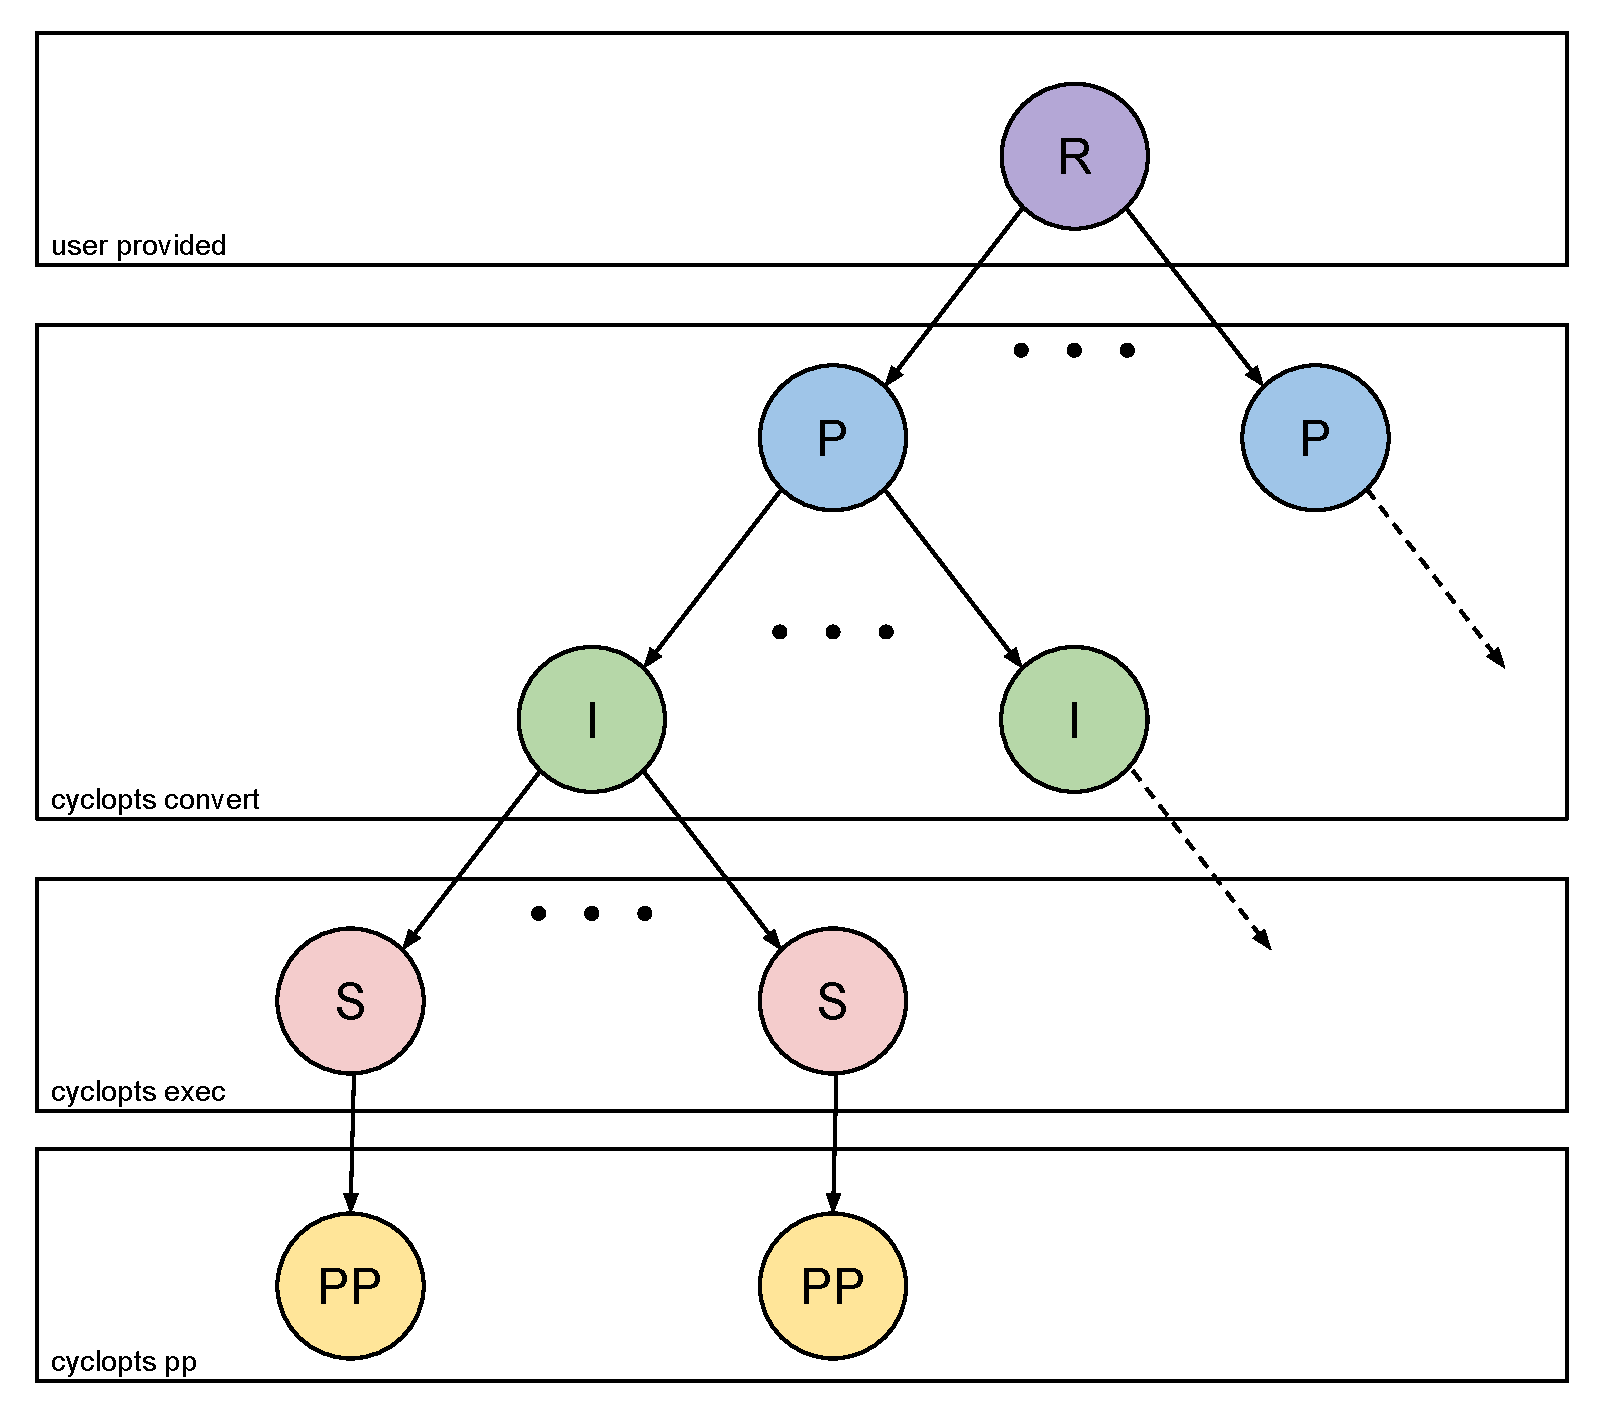
\includegraphics[width=\textwidth]{./backmatter/figs/cyclopts_tree_cli.pdf}
    \caption[]{
      \label{fig:lopts_cli}
      The Cyclopts object tree structure is shown with boxes around each group
      of objects that are created given a CLI call. Note that the root node is
      determined from user-provided input.}
  \end{center}
\end{figure}

\section{Remote Execution}

In order to execute Cyclopts on a Condor system, the submit node must contain
the Cyclopts environment. That operation is supported by the \code{cyclopts cde}
CLI, presented in Listing \ref{lst:loptscde}. A job, the input of which is an
instance database, can be submitted using \code{cyclopts condor-submit}. Upon
completion, results can be collected with \code{cyclopts condor-collect}. The
arguments for both are shown in Listings \ref{lst:loptscondor-submit} and
\ref{lst:loptscondor-collect}.

\lstinputlisting[
  style=BashOutputStyle,
  keywordstyle=\ttfamily,
  caption={CLI options for \code{cyclopts cde}.}, 
  label=lst:loptscde]{./backmatter/listings/cde}

\lstinputlisting[
  style=BashOutputStyle,
  keywordstyle=\ttfamily,
  caption={CLI options for \code{cyclopts condor-submit}.}, 
  label=lst:loptscondor-submit]{./backmatter/listings/condor-submit}

\lstinputlisting[
  style=BashOutputStyle,
  keywordstyle=\ttfamily,
  caption={CLI options for \code{cyclopts condor-collect}.}, 
  label=lst:loptscondor-collect]{./backmatter/listings/condor-collect}

\end{appendices}

%% McBride is a very nice style (some version is included in this distribution)
\bibliographystyle{mcbride}
\bibliography{./bibs/refs,./bibs/simulators,./bibs/benchmarks,./bibs/cosi,./bibs/abm-supply-chain,./bibs/blending}%,./chapters/litreview/refs}

%% Want an index?  Neither did I.
%\printindex

\end{document}
